\documentclass{article}

\usepackage{arxiv}

\usepackage[utf8]{inputenc} % allow utf-8 input
\usepackage[T1]{fontenc}    % use 8-bit T1 fonts
\usepackage{hyperref}       % hyperlinks
\usepackage{url}            % simple URL typesetting
\usepackage{booktabs}       % professional-quality tables
\usepackage{amsfonts}       % blackboard math symbols
\usepackage{nicefrac}       % compact symbols for 1/2, etc.
\usepackage{microtype}      % microtypography
\emergencystretch=1em       % suppress underfull hbox warnings
\usepackage{lipsum}         % Can be removed after putting your text content
\usepackage{graphicx}
\usepackage{natbib}
\usepackage{doi}
\usepackage{amsmath}
\usepackage{cleveref}       % smart cross-referencing (must be after amsmath)
\usepackage{ulem}
\usepackage{tikz}
\usetikzlibrary{positioning, arrows.meta, fit, backgrounds, shapes.geometric, decorations.pathreplacing}
\usepackage{amsthm}
\usepackage{algorithm}
\usepackage{algpseudocode}
\usepackage{placeins}
\usepackage{listings}
\lstset{
  language=Python,
  basicstyle=\ttfamily\footnotesize,
  keywordstyle=\bfseries\color{blue!70!black},
  commentstyle=\itshape\color{gray},
  stringstyle=\color{red!60!black},
  breaklines=true,
  frame=single,
  framerule=0.4pt,
  rulecolor=\color{gray!40},
  xleftmargin=1em,
  xrightmargin=0.5em,
  aboveskip=0.8em,
  belowskip=0.5em,
  showstringspaces=false,
}
\usepackage{xcolor}

\theoremstyle{definition}
\newtheorem{definition}{Definition}[section]
\newtheorem{remark}{Remark}[section]

% Notation shorthands
\newcommand{\LT}{\mathbf{LT}}
\newcommand{\MD}{\mathbf{MD}}
\newcommand{\BBox}{\mathcal{B}}
\newcommand{\Nodes}{\mathcal{N}}
\newcommand{\Spans}{\mathcal{S}}

\newcommand{\todo}{\textcolor{red}{TODO}}

\title{Parsed Page eXplorer (PPX): A Tool Towards Agentic Human Knowledge Distillation}

% Here you can change the date presented in the paper title
\date{April, 2026}
% Or remove it
%\date{}

\newif\ifuniqueAffiliation
% Comment to use multiple affiliations variant of author block
\uniqueAffiliationtrue

\ifuniqueAffiliation % Standard variant of author block
\author{
  {Levi Willms}
  \thanks{
    This document is a partial fulfillment of the requires for the Undergraduate honours thesis in Computer Science.
  } \\
  Computer Science, Faculty of Science\\
  Ontario Tech University\\
  Oshawa, ON \\
  \texttt{levi.willms@ontariotechu.net} \\
  \And
  {Ken Pu (\textsc{Supervisor})} \\
  Computer Science, Faculty of Science\\
  Ontario Tech University\\
  Oshawa, ON \\
  \texttt{ken.pu@ontariotechu.ca} \\
}
\else
% Multiple affiliations variant of author block
\usepackage{authblk}
\renewcommand\Authfont{\bfseries}
\setlength{\affilsep}{0em}
% box is needed for correct spacing with authblk
\newbox{\orcid}\sbox{\orcid}{\includegraphics[scale=0.06]{orcid.pdf}}
\author[1]{%
  \href{https://orcid.org/0000-0000-0000-0000}{\usebox{\orcid}\hspace{1mm}David S.~Hippocampus\thanks{\texttt{hippo@cs.cranberry-lemon.edu}}}%
}
\author[1,2]{%
  \href{https://orcid.org/0000-0000-0000-0000}{\usebox{\orcid}\hspace{1mm}Elias D.~Striatum\thanks{\texttt{stariate@ee.mount-sheikh.edu}}}%
}
\affil[1]{Department of Computer Science, Cranberry-Lemon University, Pittsburgh, PA 15213}
\affil[2]{Department of Electrical Engineering, Mount-Sheikh University, Santa Narimana, Levand}
\fi

% Uncomment to override  the `A preprint' in the header
\renewcommand{\headeright}{Honours thesis}
\renewcommand{\undertitle}{}
\renewcommand{\shorttitle}{}

%%% Add PDF metadata to help others organize their library
%%% Once the PDF is generated, you can check the metadata with
%%% $ pdfinfo template.pdf
\hypersetup{
  pdftitle={Multimodal Document Alignment: Bridging Visual Layout Trees and OCR-Extracted Markdown},
  pdfsubject={Document understanding, layout analysis, multimodal alignment},
  pdfauthor={Levi Willms; Ken Pu},
  pdfkeywords={document understanding, layout analysis, OCR, sequence alignment, multimodal document processing},
}

\begin{document}
\maketitle

\begin{abstract}
      Navigating the boundaries between vast document spaces ---
      textbooks, papers, articles --- and the abstract concepts they
      express is a grand challenge of \emph{agentic knowledge
            distillation}.  To help humans learn faster, AI agents need
      specialized tools to traverse the layers between raw information
      and actionable knowledge.  A critical missing link in this stack
      is the exact alignment between raw source documents and the
      structured text (Markdown) that downstream agents consume.
      Without such provenance, agents that translate raw data into
      concepts cannot verify, cite, or retrieve the evidence behind
      their own claims.

      This thesis addresses that bottleneck through the \emph{Parsed
            Page eXplorer} (\texttt{ppx}), a foundational tool that
      establishes strict alignment between a document page and its
      Markdown transcription.  \texttt{ppx} treats a document as two
      complementary representations: a hierarchical \emph{Layout Tree}
      $\LT$ of labeled bounding boxes produced by a layout analyzer,
      and a \emph{Markdown document} $\MD$ produced by OCR over the
      same page.  The load-bearing contribution is a mapping between
      them that assigns each visual node a contiguous span of $\MD$
      together with its semantic provenance.  This mapping lets agents
      move seamlessly between documents and information without losing
      track of where a given fragment came from.

      The thesis develops this idea in three parts.  First, we give a
      set-theoretic formulation of multimodal alignment that separates
      the four-level Layout Tree from the Markdown AST and casts
      alignment as a pair of partial injective functions scored by
      semantic similarity.  Second, we realize the model as a
      composable, embedding-based hierarchical aligner --- max-weight
      bipartite matching over cosine similarities of Sentence-BERT
      embeddings, solved via the Jonker--Volgenant
      shortest-augmenting-path algorithm at both block and line
      granularities --- and package it as a type-safe Python
      implementation on PaddleOCR / PPStructure\,V3 with a
      client/server architecture for interactive AI-assisted document
      reading.  Third, we quantify alignment quality on a 130-page
      corpus across six academic documents, measure degradation under
      controlled OCR-noise injection, and characterize a staircase
      structure of precision / recall / $F1$ collapse with increasing
      corruption.  Together these contributions provide the navigation
      mechanism between documents and information that agent-driven
      knowledge distillation requires.
\end{abstract}

% keywords can be removed
\keywords{agentic knowledge distillation \and document understanding \and
      layout analysis \and OCR \and sequence alignment \and
      multimodal document processing \and PaddleOCR \and
      Parsed Page eXplorer}

%% ---------------------------------------------------------------
\section{Introduction}
\label{sec:intro}
%% ---------------------------------------------------------------

\paragraph{The grand challenge: agentic knowledge distillation.}
Human knowledge lives across a vast \emph{document space} --- textbooks,
scientific papers, technical manuals, and online articles --- that a
single human reader can only ever traverse a small fraction of.  The
ambition of \emph{agentic knowledge distillation} is to enlist AI
agents as collaborators in this traversal: agents that read
documents on our behalf, extract the information they contain, and
refine that information into the concepts and abstractions a human
learner can act on.  The payoff is compounding: if an agent can
reliably move from a page of text to a citable fact, and from a
collection of facts to a coherent summary, the rate at which humans
turn raw documents into understanding is no longer bounded by how
quickly any one of us can read.

\paragraph{Three layers an agent must cross.}
The obstacle to this program is that agents must continually
traverse the boundaries between three qualitatively different
representations of the same content.  At the bottom sits the
\emph{document}: a page image or PDF, with visual structure
(titles, paragraphs, tables, figures) but no addressable text.  In
the middle sits \emph{information}: a linearized textual
transcription --- typically Markdown produced by an OCR pipeline ---
that is directly consumable by a language model but has lost its
spatial grounding.  At the top sits \emph{concepts}: abstractions
and claims formed from the information but disconnected from the
documents that justify them.  An agent that can freely cross these
boundaries can cite back to the page that supports a claim, verify a
fact against a figure, or refuse an answer when the evidence is
thin.  An agent that cannot remains a sophisticated guesser.

\paragraph{The missing rung: document $\leftrightarrow$ information.}
The weakest rung on this ladder is the one between \emph{documents}
and \emph{information} --- specifically, the exact correspondence
between the visual structure of a page and the Markdown extracted
from it.  Optical character recognition reduces a document image to
a linearized text stream, discarding the spatial structure that a
reader uses to navigate a page \cite{ieee2025systematic}.  Document
layout analysis, in parallel, recovers that spatial structure as a
hierarchy of labeled bounding boxes
\cite{PPDocLayout, wang2024dlaformer}, but says nothing about the
textual content those boxes contain.  Modern toolkits such as
PaddleOCR / PPStructure\,V3 \cite{PaddleOCR30} produce \emph{both}
views of the same page, yet offer no principled correspondence
between them.  Downstream agentic tasks --- retrieval-augmented
generation over documents, AI-assisted reading, table and formula
grounding --- demand exactly that correspondence, because it is
precisely what lets an agent point to \emph{where} in the document a
given piece of information came from.

\paragraph{The Parsed Page eXplorer.}
This thesis introduces the \emph{Parsed Page eXplorer} (\texttt{ppx}),
a foundational tool built explicitly to be the navigation mechanism
between documents and information.  Given a Layout Tree $\LT$
produced by a layout analyzer and a Markdown document $\MD$ produced
by an OCR engine, \texttt{ppx} assigns to each visual token in $\LT$
a contiguous span of $\MD$ that reproduces its transcription,
together with the similarity score that justified the match.  The
resulting data structure --- a hierarchical mapping from visual nodes
to Markdown spans with attached confidence --- is the \emph{semantic
      provenance} an agent needs: every fragment of extracted
information remains tethered to the visual region of the source
document it was distilled from.  We are deliberate in framing this
as a \emph{mechanism}, not a model.  \texttt{ppx} does not attempt
to generate the concepts and abstractions at the top of the ladder;
it ensures that whichever agent does can always trace a concept back
through information to its original document.

\paragraph{The layout--text alignment problem.}
Stripped of the agentic framing, the technical problem \texttt{ppx}
solves is the \emph{layout--text alignment problem}: given
$\LT$ and $\MD$, produce a mapping
$\phi : \Nodes \to \Spans_{\MD}$ that respects the four-level
containment structure of $\LT$ and the character-span semantics of
$\MD$.  Neither modality alone carries enough information to drive
structured document understanding; the alignment is the load-bearing
representation that makes both useful together.  Despite its
practical importance, the problem has lacked both a crisp formal
statement and an established evaluation protocol in the literature.

\paragraph{What this thesis contributes.}
\begin{itemize}
      \item A \textbf{set-theoretic formulation} of multimodal alignment
            (\cref{sec:formal}) that separates the four-level Layout Tree
            from the Markdown AST and poses alignment as a pair of partial
            injective functions scored by semantic similarity.
      \item A \textbf{composable pipeline} (\cref{sec:algo,sec:impl}) ---
            the \texttt{ppx} system --- realizing the model through
            sentence-embedding encoding of both modalities, hierarchical
            max-weight bipartite matching via the Jonker--Volgenant
            algorithm at block and line granularities, and a type-safe
            client / server architecture for interactive AI-assisted
            document reading.
      \item An \textbf{empirical benchmark} (\cref{sec:bench}) measuring
            alignment quality and robustness over a 130-page, six-document
            corpus, including a noise-injection study that exposes a
            \emph{staircase} degradation pattern in precision, recall, and
            $F1$ as OCR noise increases.
\end{itemize}

\paragraph{Scope.}
We restrict attention to English-language academic PDFs rendered by
PaddleOCR / PPStructure\,V3; multi-script, handwritten, and
historical material are out of scope.  Likewise, the upper rung of
the ladder --- concepts and abstractions formed from the extracted
information --- is the domain of whichever agent consumes
\texttt{ppx}'s output and is outside the scope of this thesis.

\paragraph{Organization.}
\Cref{sec:related} surveys OCR, layout analysis, reading-order
recovery, and the small prior literature on cross-modal alignment of
visual tokens and text.  \Cref{sec:formal} formalizes the alignment
problem set-theoretically.  \Cref{sec:algo} presents the
embedding-based hierarchical aligner and its two constituent
algorithms.  \Cref{sec:impl} describes the three-package
implementation (\texttt{ppx-ocr}, \texttt{ppx-align},
\texttt{ppx-svelte}) that makes up the \texttt{ppx} toolkit.
\Cref{sec:bench} reports empirical alignment quality, noise
robustness, and precision / recall / $F1$ degradation.
\Cref{sec:conclusion} concludes with limitations and future work.

%% ---------------------------------------------------------------
\section{Related Work}
\label{sec:related}
%% ---------------------------------------------------------------

The \texttt{ppx} toolkit sits at the intersection of four research
threads: optical character recognition as the text backbone, document
layout analysis as the structural backbone, reading-order and
structure extraction as adjacent end-to-end approaches, and the
comparatively small literature on cross-modal alignment between
visual tokens and text.  We survey each in turn and close by naming
the gap \texttt{ppx} occupies.

\subsection{Optical Character Recognition}

Modern OCR is the product of a long transition from rule-based
template matching to deep-learning detectors and sequence decoders.
Classical engines such as \texttt{Tesseract} \cite{smith2007tesseract}
began with per-glyph templates and progressed to LSTM-based
recognition in their later releases; contemporary systems pair
fully-convolutional text detectors with attention-based or
transformer-based recognizers.  The breadth of this progression is
cataloged in recent systematic reviews of the field
\cite{ieee2025systematic}.

For \texttt{ppx} the backbone of interest is the \emph{PaddleOCR}
family.  PP-OCRv3 \cite{PaddleOCRv3} is the lightweight
detector-recognizer pair that supplies line- and word-level
transcriptions.  PaddleOCR\,3.0 \cite{PaddleOCR30} extends this core
with the PP-StructureV3 layout analyzer and a Markdown-first
document parsing front-end, which together give our pipeline both of
the representations it needs to align.  PaddleOCR-VL
\cite{paddleocrvl2025} is an ultra-compact vision-language model
for multilingual document parsing, relevant as a possible alternative
backend behind the same \texttt{ppx} adapters but not currently
adopted.

An orthogonal family of systems skips the OCR pipeline decomposition
altogether.  Donut \cite{kim2022donut} and Nougat
\cite{blecher2023nougat} are encoder-decoder models that emit
structured text --- JSON and Markdown respectively --- directly from
the page image, without producing intermediate bounding boxes.
These approaches are complementary rather than competing in our
setting: they produce the Markdown we would want to align against,
but they do not expose the aligned visual tokens that our
bipartite-matching pipeline requires on the other side.

\subsection{Document Layout Analysis}

\paragraph{Datasets.}  The large-scale study of document layout owes
much to two dataset efforts.  \textbf{PubLayNet}
\cite{zhong2019publaynet} automatically aligned roughly 360{,}000
PubMed Central pages with their companion XML to produce what was at
the time the largest public layout-analysis corpus.
\textbf{DocLayNet} \cite{pfitzmann2022doclaynet} contributed
$80{,}863$ \emph{human-annotated} pages across eleven categories and
diverse domains; its annotation effort (32 annotators over roughly
three months) stands as the practical scale benchmark for any
manually-supervised document corpus and is the reference point against
which we compare the modest 130-page corpus of \cref{sec:bench}.

\paragraph{Detectors.}  On the model side, PP-DocLayout
\cite{PPDocLayout} is the detector behind PP-StructureV3 and is the
direct source of the region- and block-level labels \texttt{ppx}
consumes.  DLAFormer \cite{wang2024dlaformer} formulates layout
analysis end-to-end as a set-prediction transformer, representative
of the contemporary move from pipeline-style detection to unified
sequence-to-set models.

\paragraph{Multimodal pre-trained models.}  A parallel line of work
builds pre-trained transformers that jointly ingest text, layout,
and image features.  LayoutLMv3 \cite{huang2022layoutlmv3} is
notable for including a word-patch alignment objective during
pre-training; UDOP \cite{tang2023udop} unifies vision, text, and
layout into a single generative transformer capable of document
understanding and generation.  Both are natural neighbors to our
work because both operate over text-with-layout inputs, but both
express alignment as a \emph{model-internal} pre-training signal
rather than as an externally-visible mapping between visual tokens
and Markdown spans.  The mapping we produce is designed to be
inspected, cited, and consumed by external agents --- a different
object from the one these architectures compute inside their
encoders.

\subsection{Reading Order and Structure Extraction}

\paragraph{Reading-order algorithms.}  Reading-order recovery is a
long-running sub-problem of document analysis.  Classical XY-cut
\cite{meunier2005xycut} remains the archetypal
projection-profile algorithm and the baseline against which newer
methods are measured.  LayoutReader \cite{wang2021layoutreader}
recast the problem as seq2seq prediction and released the companion
ReadingBank dataset, enabling learning-based approaches at scale.
More recent work \cite{zhang2024modeling} casts reading order as an
ordering relation learnt directly from layout signals, moving away
from explicit sequence decoding.  Reading order enters \texttt{ppx}
indirectly: PP-StructureV3 supplies a reading-order index for each
block, and our bipartite-matching formulation uses that order to
keep the per-level alignment sub-problems tractable and
well-defined.

\paragraph{Integrated parsers.}  Several recent systems merge
detection, recognition, and reading-order into a single model.
      {\'E}clair \cite{eclair2025extracting} predicts text, bounding
boxes, and semantic class in reading order as one end-to-end
forward pass.  Together with Nougat \cite{blecher2023nougat}, these
are the closest single-shot analogs to our decomposed pipeline.
The trade-off is familiar: integrated models can be optimized
jointly but expose fewer well-typed intermediates, while a
decomposed pipeline (\cref{sec:impl}) is easier to inspect, swap
components in, and benchmark stage-by-stage.

\paragraph{Structural benchmarks.}  Two recent benchmarks frame the
end-to-end problem of turning a PDF into structured Markdown.
READoc \cite{li2024readoc} evaluates PDF-to-Markdown conversion
over 2{,}233 arXiv and GitHub documents with an explicit
reading-order component; OmniDocBench
\cite{ouyang2025omnidocbench} extends benchmarking to diverse PDF
parsing with comprehensive per-element annotations.  Neither
benchmark measures \emph{token-level alignment} between visual
tokens and the extracted Markdown --- both operate at the
end-to-end output level --- which leaves the noise-injection regime
of \cref{sec:bench} complementary rather than redundant to this line
of work.

\subsection{Cross-Modal Alignment of Visual Tokens and Text}

The direct neighbors of our problem are the few lines of prior
work that explicitly address an alignment between visual and textual
representations of a document.  Each intersects our setting along
one axis but not all of them.

\paragraph{Token-patch alignment inside pre-trained models.}  The
word-patch alignment objective of LayoutLMv3
\cite{huang2022layoutlmv3} is the closest conceptual neighbor we
know of: during pre-training the model is encouraged to map masked
words to their corresponding image patches.  Two differences matter.
First, this is a \emph{pre-training} signal internal to a single
model, not a standalone aligner one can invoke at inference time on
an arbitrary OCR output.  Second, it operates at word / patch
granularity, whereas \texttt{ppx} aligns at the block- and
line-level structure of the AST.  LayoutLMv3's alignment is a
representation-learning mechanism; ours is an output artifact.

\paragraph{Scene-text alignment.}  ODM \cite{duan2024odm} proposes
a further text-image alignment objective aimed at scene-text
detection and spotting.  The setting --- unconstrained outdoor
imagery with short text strings and no layout hierarchy --- is
structurally different from the paginated-document case we study,
and the alignment problem reduces to per-instance matching rather
than to hierarchical span assignment.

\paragraph{Post-OCR string alignment.}  The post-OCR correction
literature, exemplified by work such as
\cite{martinek2019aligning}, aligns noisy OCR output against an
independent ground-truth transcript using edit distance or fuzzy
string matching.  This is character- or word-level, assumes a
reference transcript exists, and aims to \emph{correct} the OCR
output rather than to establish a correspondence between two
co-produced representations of the same page.  Structurally it sits
one rung below our problem: it aligns an OCR string against a gold
string, not a layout-tree against a Markdown AST.

\paragraph{Positioning.}  To the best of our knowledge, no prior
work (i) aligns four-level layout tokens to a structured Markdown
AST produced by the same OCR pipeline, or (ii) does so as
max-weight bipartite matching over sentence-embedding cosine
similarities at both block and line granularities.  The formulation
of \cref{sec:formal} and the algorithms of \cref{sec:algo}
therefore occupy a gap between the model-internal alignment
objectives of the Document-AI literature and the string-level
alignment of the post-OCR correction tradition.  Framing \texttt{ppx}
as the navigation mechanism between documents and information
(\cref{sec:intro}) is intended partly as a research-program
statement: the alignment artifact itself, not the model that
produced it, is the primary object of study.

%% ---------------------------------------------------------------
\section{Problem Formulation}
\label{sec:formal}
%% ---------------------------------------------------------------

We give a set-theoretic account of the two representations of a page and
cast \emph{multimodal alignment} as a mapping between them.  Throughout
this section, $\Lambda$ denotes a finite set of layout labels and $\Sigma$
the Unicode character set.

\subsection{Document Representations}

\begin{definition}[Raster Document]
      A \emph{raster document} is a finite sequence of page images
      $D = \langle d_1, d_2, \ldots, d_P \rangle$, where each page
      $d_p \in \mathbb{R}^{H \times W \times 3}$ is an RGB image.  All
      subsequent definitions apply to a single page; the page index $p$ is
      dropped for brevity.
\end{definition}

\begin{definition}[Bounding Box]
      A \emph{bounding box} over label set $\Lambda$ is a tuple
      \[
            b = (x_0,\, y_0,\, x_1,\, y_1,\, \lambda)
            \;\in\; \mathbb{N}^4 \times \Lambda,
      \]
      with top-left corner $(x_0, y_0)$, bottom-right corner $(x_1, y_1)$, and
      semantic label $\lambda \in \Lambda$ (e.g.\ \texttt{paragraph},
      \texttt{figure}, \texttt{table}).  The \emph{area} of $b$ is
      $\mathrm{area}(b) = (x_1 - x_0)(y_1 - y_0)$.
\end{definition}

\begin{definition}[Containment]
      Bounding box $b'$ is \emph{contained in} $b$, written $b' \sqsubseteq b$,
      if and only if
      \[
            \frac{\mathrm{area}(b \cap b')}{\mathrm{area}(b')} \;\ge\; \tau,
      \]
      for a fixed tolerance $\tau \in (0, 1]$, where $b \cap b'$ denotes the
      rectangular intersection.  We use $\tau = 0.8$ throughout.
\end{definition}

\subsection{Visual Tokens and the Layout Tree}

The layout analyzer \cite{PPDocLayout, PaddleOCR30} parses a page into a
four-level hierarchy of labeled bounding boxes.

\begin{definition}[Visual Token Layers]
      A page is analyzed into four ordered token layers:
      \begin{itemize}
            \item $R = \{r_i\}$ --- \emph{region} bounding boxes (coarsest granularity)
            \item $K = \{k_j\}$ --- \emph{block} bounding boxes, each carrying a
                  reading-order index $\mathrm{ord}(k_j) \in \mathbb{N}$
                  \cite{zhang2024modeling}
            \item $\mathcal{L} = \{\ell_m\}$ --- \emph{line} bounding boxes, sorted by $y_0$
            \item $W = \{w_n\}$ --- \emph{word} bounding boxes, grouped by line membership
      \end{itemize}
      Each visual token $v$ is additionally annotated with its OCR transcription
      $\mathrm{content}(v) \in \Sigma^{*}$.
\end{definition}

\begin{definition}[Layout Tree]
      \label{def:lt}
      The \emph{Layout Tree} $\LT$ is a rooted tree with node set
      $\Nodes = R \cup K \cup \mathcal{L} \cup W$ and edges given by containment:
      \[
            \mathrm{parent}(v) = \arg\max_{u \in \mathrm{level}(v)-1}
            \frac{\mathrm{area}(u \cap v)}{\mathrm{area}(v)},
      \]
      where $\mathrm{level}(v) \in \{0,1,2,3\}$ denotes region, block, line, and
      word.  Children of each internal node are sorted by reading order.
      See \cref{fig:layout-tree}.
\end{definition}

\begin{figure}[h]
      \centering
      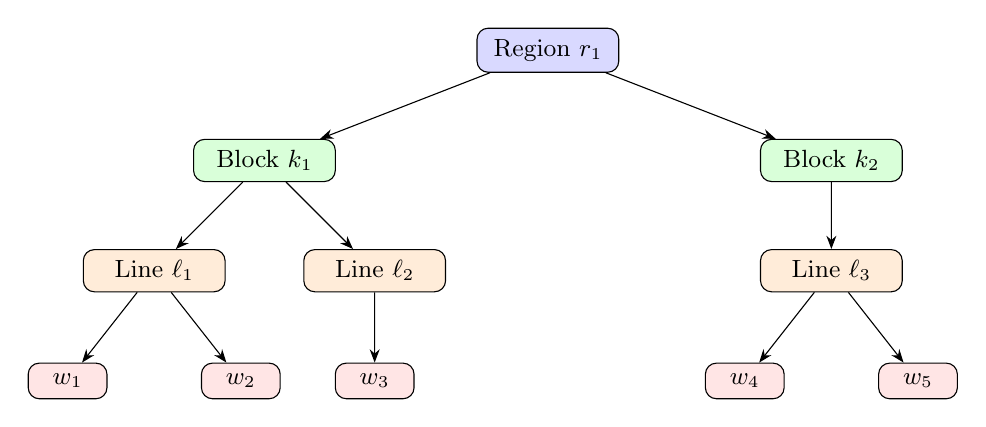
\begin{tikzpicture}[
                  level distance=14mm,
                  level 1/.style={sibling distance=72mm},
                  level 2/.style={sibling distance=28mm},
                  level 3/.style={sibling distance=22mm},
                  every node/.style={draw, rounded corners, font=\small,
                              inner sep=4pt, minimum width=18mm},
                  region/.style={fill=blue!15},
                  block/.style={fill=green!15},
                  line/.style={fill=orange!15},
                  word/.style={fill=red!10, minimum width=10mm},
                  edge from parent/.style={draw, ->, >=Stealth},
            ]
            \node[region] {Region $r_1$}
            child { node[block] {Block $k_1$}
                        child { node[line] {Line $\ell_1$}
                                    child { node[word] {$w_1$} }
                                    child { node[word] {$w_2$} }
                              }
                        child { node[line] {Line $\ell_2$}
                                    child { node[word] {$w_3$} }
                              }
                  }
            child { node[block] {Block $k_2$}
                        child { node[line] {Line $\ell_3$}
                                    child { node[word] {$w_4$} }
                                    child { node[word] {$w_5$} }
                              }
                  };
      \end{tikzpicture}
      \caption{Schematic of the Layout Tree $\LT$.  Colors denote hierarchy
            levels: \textcolor{blue!60}{region} $\supset$
            \textcolor{green!60!black}{block} $\supset$
            \textcolor{orange!80!black}{line} $\supset$
            \textcolor{red!60}{word}.
            Children within each level are ordered by reading order.}
      \label{fig:layout-tree}
\end{figure}

\subsection{Text Tokens and the Markdown Document}

The OCR engine \cite{PaddleOCR30, eclair2025extracting} produces a single
Markdown string $\MD \in \Sigma^{*}$.  Parsing $\MD$ with a Markdown parser
yields a structured view suitable for alignment.

\begin{definition}[Markdown Document and AST]
      A \emph{parsed Markdown document} is a tuple
      \[
            \MD = (\mu,\; \mathcal{A},\; \sigma,\; \omega),
      \]
      where
      \begin{itemize}
            \item $\mu \in \Sigma^{*}$ is the raw Markdown string;
            \item $\mathcal{A} = \langle a_0, a_1, \ldots, a_{N-1}\rangle$ is the
                  ordered list of leaf \emph{AST nodes} (paragraphs, list items,
                  headings, code blocks, etc.) in document order;
            \item $\sigma : \mathcal{A} \to \mathbb{N} \times \mathbb{N}$ assigns to
                  each AST node $a_i$ a character span
                  $\sigma(a_i) = [s_i, e_i) \subseteq [0, |\mu|)$;
            \item $\omega : \mathcal{A} \to (\mathbb{N}\times\mathbb{N})^{*}$
                  assigns to each AST node $a_i$ an ordered list of
                  \emph{word spans} $\omega(a_i) = \langle[p_{i,1}, q_{i,1}), \ldots\rangle$
                  relative to the node's content.
      \end{itemize}
      See \cref{fig:text-tokens}.
\end{definition}

\begin{definition}[AST-Node Range]
      An \emph{AST-node range} is a half-open integer interval
      $[i, j) \subseteq [0, N)$ selecting the contiguous sub-sequence
      $\mathcal{A}[i{:}j]$ of leaf nodes.  Its induced character span is
      $\widetilde{\sigma}([i,j)) = [s_i,\; e_{j-1}) \subseteq [0, |\mu|)$.
      Denote by $\Spans_{\mathcal{A}}$ the set of all such AST-node ranges.
\end{definition}

\begin{definition}[Word-Bounded Character Sub-Span]
      For any AST-node range $[i,j)$, a \emph{word-bounded sub-span} is a
      character interval $[c_{\text{s}}, c_{\text{e}}) \subseteq
            \widetilde{\sigma}([i,j))$ whose endpoints coincide with word-span
      boundaries in $\bigcup_{k = i}^{j-1}\omega(a_k)$.  Denote by
      $\Spans_{W}$ the set of all such sub-spans.
\end{definition}

\begin{figure}[h]
      \centering
      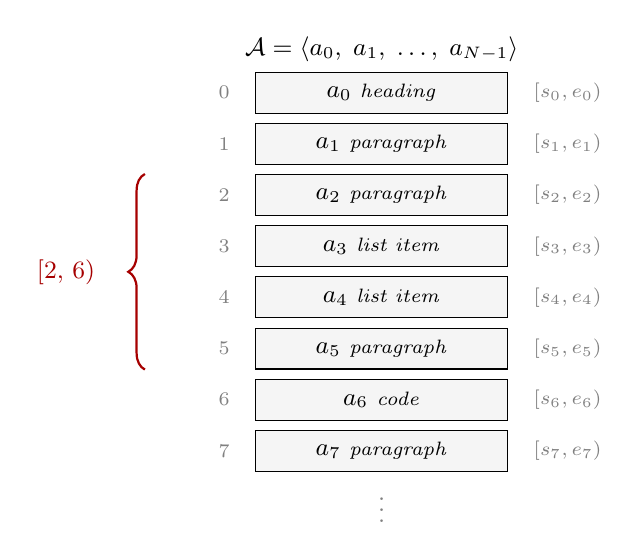
\begin{tikzpicture}[
                  tok/.style={draw, fill=gray!8, font=\small, inner sep=3pt,
                              minimum height=0.52cm, minimum width=3.2cm, text centered},
            ]
            % Header
            \node[font=\small\bfseries] (hdr) at (0, 0.55)
            {$\mathcal{A} = \langle a_0,\; a_1,\; \ldots,\; a_{N-1} \rangle$};

            % AST-node boxes stacked vertically
            \foreach \i/\lab/\span in {
            0/$a_0$ {\scriptsize\textit{heading}}/{\scriptsize$[s_0,e_0)$},
                  1/$a_1$ {\scriptsize\textit{paragraph}}/{\scriptsize$[s_1,e_1)$},
                  2/$a_2$ {\scriptsize\textit{paragraph}}/{\scriptsize$[s_2,e_2)$},
                  3/$a_3$ {\scriptsize\textit{list item}}/{\scriptsize$[s_3,e_3)$},
                  4/$a_4$ {\scriptsize\textit{list item}}/{\scriptsize$[s_4,e_4)$},
                  5/$a_5$ {\scriptsize\textit{paragraph}}/{\scriptsize$[s_5,e_5)$},
                  6/$a_6$ {\scriptsize\textit{code}}/{\scriptsize$[s_6,e_6)$},
                  7/$a_7$ {\scriptsize\textit{paragraph}}/{\scriptsize$[s_7,e_7)$}}{
                  \node[tok] (T\i) at (0, {-\i*0.65}) {\lab};
                  \node[font=\scriptsize, gray, left=2mm of T\i] {\i};
                  \node[font=\scriptsize, gray, right=2mm of T\i] {\span};
                  }

                  % Brace showing an example AST-node range [2,6)
                  \draw[decorate,
                        decoration={brace, amplitude=6pt, mirror},
                        thick, red!65!black]
                  ([xshift=-1.4cm]T2.north west) --
                  ([xshift=-1.4cm]T5.south west)
                  node[midway, left=5mm, font=\small, red!65!black] {$[2,\,6)$};

            \node[font=\small, gray] at (0, {-8*0.65}) {$\vdots$};
      \end{tikzpicture}
      \caption{The AST-node sequence $\mathcal{A}$ obtained by parsing the
      OCR-generated Markdown $\MD$.  Nodes are indexed $0 \ldots N{-}1$ (left)
      and each carries a character span $[s_i, e_i) \subseteq [0, |\mu|)$
      (right).  The red brace marks an example \emph{AST-node range} $[2,6)$,
      inducing the contiguous character span $[s_2, e_5)$ of $\mu$.}
      \label{fig:text-tokens}
\end{figure}

\subsection{The Alignment Problem}

The alignment problem pairs visual tokens with Markdown at two granularities:
blocks to AST-node ranges, and lines to word-bounded character sub-spans
within each block's range.  We formalize both as \emph{partial} functions
with a rejection regime governed by a similarity threshold.

\begin{definition}[Semantic Embedding]
      A \emph{semantic embedding} is a function
      $\varepsilon : \Sigma^{*} \to \mathbb{R}^{d}$ that maps a string to a
      $d$-dimensional unit vector.  We realize $\varepsilon$ with a
      Sentence-BERT encoder \cite{reimers2019sbert, wang2020minilm}.
\end{definition}

\begin{definition}[Similarity Function]
      Given embedding $\varepsilon$, the \emph{similarity} between a visual
      token $v$ with transcription $\mathrm{content}(v)$ and a text fragment
      $y \in \Sigma^{*}$ is the cosine similarity of their embeddings:
      \[
            \mathrm{sim}(v,\, y) \;=\;
            \frac{\varepsilon(\mathrm{content}(v)) \cdot \varepsilon(y)}
            {\lVert \varepsilon(\mathrm{content}(v)) \rVert\,
                  \lVert \varepsilon(y) \rVert}
            \;\in\; [-1, 1].
      \]
\end{definition}

\begin{definition}[Block Alignment]
      \label{def:block-align}
      Let $K \subseteq \Nodes$ be the set of block visual tokens and
      $\Spans_{\mathcal{A}}$ the AST-node ranges of $\MD$.  A \emph{block
            alignment} is a partial injective function
      \[
            \phi_K \;:\; K \;\rightharpoonup\; \Spans_{\mathcal{A}}.
      \]
      Given threshold $\theta \in [-1, 1]$, $\phi_K$ is \emph{valid} if, for
      every $k \in \mathrm{dom}(\phi_K)$,
      $\mathrm{sim}(k,\, \mu[\widetilde{\sigma}(\phi_K(k))]) \ge \theta$.
\end{definition}

\begin{definition}[Line Alignment]
      \label{def:line-align}
      For each block $k \in \mathrm{dom}(\phi_K)$, let $L_k \subseteq \Nodes$
      be its line children in $\LT$ and let $\Spans_{W}^{(k)}$ be the set of
      word-bounded sub-spans of the character range
      $\widetilde{\sigma}(\phi_K(k))$.  A \emph{line alignment conditioned on
            $k$} is a partial injective function
      \[
            \phi_\ell^{(k)} \;:\; L_k \;\rightharpoonup\; \Spans_{W}^{(k)},
      \]
      valid under threshold $\theta$ analogously to \cref{def:block-align}.
\end{definition}

\begin{definition}[Multimodal Alignment]
      The \emph{multimodal alignment problem} is, given $\LT$, $\MD$,
      embedding $\varepsilon$, and threshold $\theta$, to compute the pair
      $(\phi_K^{*},\, \{\phi_\ell^{(k)*}\}_{k\in\mathrm{dom}(\phi_K^{*})})$ that
      maximizes the total similarity score
      \[
            \sum_{k \in \mathrm{dom}(\phi_K)}
            \!\!\mathrm{sim}(k, \mu[\widetilde{\sigma}(\phi_K(k))])
            \;+\;
            \sum_{k}\;\sum_{\ell \in \mathrm{dom}(\phi_\ell^{(k)})}
            \!\!\mathrm{sim}(\ell,\, \mu[\phi_\ell^{(k)}(\ell)])
      \]
      over all valid alignments.  See \cref{fig:alignment}.
\end{definition}

\begin{figure}[h]
      \centering
      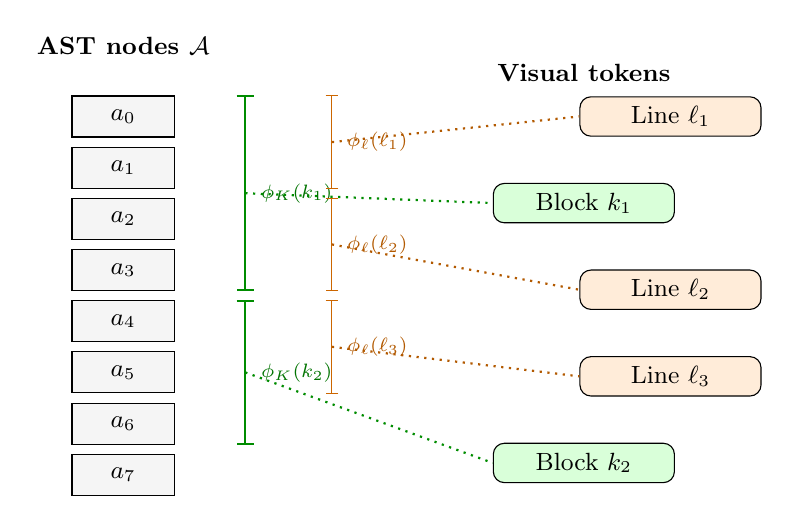
\begin{tikzpicture}[
                  nd/.style={draw, rounded corners, font=\small, inner sep=3pt,
                              minimum height=0.50cm, minimum width=2.3cm, text centered},
                  tok/.style={draw, fill=gray!8, font=\small, inner sep=2pt,
                              minimum height=0.52cm, minimum width=1.3cm, text centered},
                  conn/.style={dotted, thick},
            ]

            % ---- AST-node column (LEFT) ----
            \foreach \i/\lab in {
                        0/$a_0$, 1/$a_1$, 2/$a_2$, 3/$a_3$,
                        4/$a_4$, 5/$a_5$, 6/$a_6$, 7/$a_7$}{
                        \node[tok] (T\i) at (0.55, {-\i*0.65}) {\lab};
                  }
            \node[font=\small\bfseries, above=4mm of T0] {AST nodes $\mathcal{A}$};

            % ---- Block-range brackets (GREEN) ----
            % Block k_1 matched to AST range [0,4)
            \draw[|-|, thick, green!55!black]
            (2.1,  0.27) -- (2.1, {-3*0.65-0.27})
            node[midway, right=2pt, font=\scriptsize, green!45!black] {$\phi_K(k_1)$};
            % Block k_2 matched to AST range [4,7)
            \draw[|-|, thick, green!55!black]
            (2.1, {-4*0.65+0.27}) -- (2.1, {-6*0.65-0.27})
            node[midway, right=2pt, font=\scriptsize, green!45!black] {$\phi_K(k_2)$};

            % ---- Line sub-span brackets (ORANGE, inside k_1) ----
            \draw[|-|, orange!80!black]
            (3.2,  0.27) -- (3.2, {-1*0.65-0.27})
            node[midway, right=2pt, font=\scriptsize, orange!70!black] {$\phi_\ell(\ell_1)$};
            \draw[|-|, orange!80!black]
            (3.2, {-2*0.65+0.27}) -- (3.2, {-3*0.65-0.27})
            node[midway, right=2pt, font=\scriptsize, orange!70!black] {$\phi_\ell(\ell_2)$};
            % Line sub-span inside k_2
            \draw[|-|, orange!80!black]
            (3.2, {-4*0.65+0.27}) -- (3.2, {-5*0.65-0.27})
            node[midway, right=2pt, font=\scriptsize, orange!70!black] {$\phi_\ell(\ell_3)$};

            % ---- Node column (RIGHT) ----
            \node[nd, fill=orange!15] (L1) at (7.5,  0.00) {Line $\ell_1$};
            \node[nd, fill=green!15]  (K1) at (6.4, -1.10) {Block $k_1$};
            \node[nd, fill=orange!15] (L2) at (7.5, -2.20) {Line $\ell_2$};
            \node[nd, fill=orange!15] (L3) at (7.5, -3.30) {Line $\ell_3$};
            \node[nd, fill=green!15]  (K2) at (6.4, -4.40) {Block $k_2$};
            \node[font=\small\bfseries] at (6.4, 0.55) {Visual tokens};

            % ---- Connectors ----
            \draw[conn, green!55!black]  (2.1, {-1.5*0.65}) -- (K1.west);
            \draw[conn, green!55!black]  (2.1, {-5.0*0.65}) -- (K2.west);
            \draw[conn, orange!70!black] (3.2, {-0.5*0.65}) -- (L1.west);
            \draw[conn, orange!70!black] (3.2, {-2.5*0.65}) -- (L2.west);
            \draw[conn, orange!70!black] (3.2, {-4.5*0.65}) -- (L3.west);

      \end{tikzpicture}
      \caption{The multimodal alignment $(\phi_K, \phi_\ell)$ as a pair of
            mappings.  At the \textcolor{green!60!black}{block level}, each visual
            block is matched to an AST-node range of $\mathcal{A}$
            (green brackets).  At the \textcolor{orange!80!black}{line level},
            each line within a matched block is matched to a word-bounded
            character sub-span inside that block's range (orange brackets).
            Dotted arrows depict the assignment.  The alignment is partial: a
            visual token with no candidate scoring above $\theta$ is left unmatched.}
      \label{fig:alignment}
\end{figure}

\begin{remark}
      Unlike interval-partition formulations, $\phi_K$ and $\phi_\ell^{(k)}$
      are neither required to cover their parent span nor to assign every
      visual token: thresholding admits rejection, and bipartite injectivity
      prevents reuse of the same text fragment.  Each level reduces to a
      \emph{max-weight bipartite matching} problem, solved in \cref{sec:algo}.
\end{remark}

%% ---------------------------------------------------------------
\section{Alignment Algorithms}
\label{sec:algo}
%% ---------------------------------------------------------------

This section operationalizes the multimodal alignment problem of
\cref{def:block-align,def:line-align} as a sequence of concrete
algorithms.  The pipeline proceeds in three logical stages.  First,
an \emph{encode} stage lifts visual tokens and Markdown fragments into
a shared semantic vector space through a Sentence-BERT encoder.
Second, a \emph{match} stage builds a bipartite cost matrix from
pairwise cosine similarities at each hierarchy level and solves the
associated max-weight assignment with the Jonker--Volgenant
shortest-augmenting-path algorithm.  Finally, a \emph{compose} stage
stacks a block-level matching over the whole page with a line-level
matching \emph{conditioned on} each matched block's AST-node range,
so that line alignment inherits the containment structure of the
Layout Tree without enforcing it through a hard constraint.  The
remainder of this section fills in each stage.

\subsection{Semantic Embeddings of Visual and Textual Tokens}
\label{sec:emb}

Both modalities are encoded with a single shared Sentence-BERT
model \cite{reimers2019sbert}, instantiated as the distilled
\texttt{all-MiniLM-L6-v2} checkpoint built on the MiniLM architecture
\cite{wang2020minilm}.  Sharing one encoder across both sides is
essential: cosine similarity is only meaningful between vectors drawn
from the same embedding space, and any mismatch between a separate
``vision'' and ``text'' encoder would have to be bridged by an
explicit projection we would then have to calibrate.  Using the same
encoder on OCR transcriptions and Markdown candidates sidesteps that
problem --- both inputs are strings over $\Sigma$ from the encoder's
perspective.

Formally, let $\varepsilon : \Sigma^{*} \to \mathbb{R}^{d}$ denote
the encoder ($d = 384$ for \texttt{all-MiniLM-L6-v2}), producing a
unit-norm dense vector for any input string.  On the \emph{visual
      side}, each visual token $v \in \Nodes$ supplies its OCR
transcription $\mathrm{content}(v)$ (recovered by PaddleOCR in the
pipeline of \cref{sec:impl}) and receives the embedding
$\mathbf{e}_v = \varepsilon(\mathrm{content}(v))$.  On the
\emph{textual side}, each candidate Markdown fragment
$y \in \Sigma^{*}$ receives $\mathbf{e}_y = \varepsilon(y)$.  At
block granularity these candidates are AST-node ranges $[i, j)$
materialized as the Markdown slice
$\mu[\widetilde{\sigma}([i, j))]$; at line granularity they are the
word-bounded sub-spans enumerated in \cref{sec:line}.

Encoding is both batched and memoized.  A single
\texttt{functools.cache}'d \texttt{get\_model} factory returns the
shared \texttt{SentenceTransformer} instance, so model-loading cost
is paid exactly once per process.  Within a page, every visual-token
content string and every candidate fragment is collected into a
single list before calling \texttt{.encode}, letting the encoder
exploit GPU-friendly batched inference rather than issuing a forward
pass per string.

\subsection{Cosine Similarity and Max-Weight Bipartite Matching}
\label{sec:match}

\paragraph{Cosine similarity matrix.}
Given query embeddings $A \in \mathbb{R}^{m \times d}$ for the visual
tokens at some level and candidate embeddings $B \in \mathbb{R}^{n
            \times d}$ for the corresponding Markdown fragments, the
\emph{similarity matrix} $S \in [-1, 1]^{m \times n}$ records the
cosine similarity of every visual-token / candidate pair:
\[
      S_{ij} \;=\; \frac{A_i \cdot B_j}{\lVert A_i\rVert\,\lVert B_j\rVert}.
\]
In practice, because the MiniLM checkpoint emits unit-norm embeddings,
$S$ reduces to the dot product $A B^{\top}$.  Our implementation
computes it uniformly as $S = 1 - \mathrm{cdist}(A, B, \text{cosine})$
via SciPy \cite{virtanen2020scipy}, which is robust to the rare case
in which the encoder returns non-unit vectors and costs $O(m n d)$
floating-point multiplies.

\paragraph{From similarity to bipartite matching.}
At each hierarchy level the alignment sub-problem is: select a
\emph{partial injective function} $\phi : \{0, \ldots, m{-}1\}
      \rightharpoonup \{0, \ldots, n{-}1\}$ that maximizes the total
similarity $\sum_i S_{i, \phi(i)}$.  Injectivity encodes the
requirement from \cref{def:block-align,def:line-align} that no
Markdown fragment be reused for two different visual tokens;
partiality accommodates the rejection regime introduced by the
similarity threshold below.  This is precisely the \emph{linear
      assignment problem} over the rectangular cost matrix
$C = -S$, a classical combinatorial-optimization problem solvable in
polynomial time.

We solve it with SciPy's \texttt{linear\_sum\_assignment}, which
implements the Jonker--Volgenant shortest-augmenting-path algorithm
\cite{jonker1987shortest, crouse2016implementing}.  The routine
returns two index vectors $(I, J)$ such that the pairs
$\{(I_k, J_k)\}$ form an optimal assignment.  The worst-case time
complexity is $O(\max(m, n)^3)$; in our setting $n \gg m$ (many
candidate fragments against a handful of visual tokens), so the
assignment cost is effectively cubic in $n$.  In practice the
runtimes we observe are far below the worst case because the cost
matrix is dense but dominated by a small number of high-similarity
entries per row, a regime where shortest-augmenting-path methods
terminate early.

\paragraph{Thresholded rejection.}
After the optimum has been selected, we apply a \emph{similarity
      threshold} $\theta \in [-1, 1]$: for each pair $(i, j)$ returned
by the solver, keep the edge only if $S_{i, j} \ge \theta$.  This
realizes the partial-function semantics of
\cref{def:block-align,def:line-align}: a visual token for which no
candidate scores above $\theta$ is left unmatched rather than forced
into a low-confidence assignment.  Crucially, thresholding happens
\emph{after} global optimization, so it can only prune weak edges; it
never swaps a high-scoring edge for a weaker one.  The role of
$\theta$ as a precision / recall knob is discussed in
\cref{sec:compose}.

\Cref{alg:match} states the complete matching primitive.  It is the
single procedure invoked at both hierarchy levels --- only the
embedding matrices and the threshold change.

\begin{algorithm}[h]
      \caption{Max-weight bipartite matching with thresholding}
      \label{alg:match}
      \begin{algorithmic}[1]
            \Require query embeddings $A \in \mathbb{R}^{m\times d}$,
            candidate embeddings $B \in \mathbb{R}^{n\times d}$,
            threshold $\theta$
            \Ensure list of triples $(i, j, s)$ with $s \ge \theta$
            \State $S \gets 1 - \mathrm{cdist}(A, B, \text{cosine})$
            \Comment{pairwise cosine similarity, $S \in \mathbb{R}^{m\times n}$}
            \State $(I, J) \gets \textsc{LinearSumAssignment}(-S)$
            \Comment{Jonker--Volgenant, maximize total similarity}
            \State $M \gets \emptyset$
            \For{$(i, j) \in \mathrm{zip}(I, J)$}
            \If{$S_{i,j} \ge \theta$}
            \State $M \gets M \cup \{(i,\, j,\, S_{i,j})\}$
            \EndIf
            \EndFor
            \State \Return $M$
      \end{algorithmic}
\end{algorithm}

\subsection{Block-Level Alignment over AST-Node Ranges}
\label{sec:block}

\paragraph{Candidate generation.}
Let $K = \{k_1, \ldots, k_m\} \subseteq \Nodes$ be the block-level
visual tokens of a page's Layout Tree.  The block-alignment stage
must decide, for each $k_i$, which contiguous chunk of the Markdown
AST transcribes it.  Because the OCR pipeline does not expose block
boundaries in the Markdown stream directly, we do not know in advance
which ranges are plausible candidates; we therefore enumerate
\emph{every} contiguous AST-node range.  Concretely, for all
$0 \le i < j \le N$ the pair $[i, j)$ identifies one candidate,
yielding $\binom{N+1}{2} = O(N^2)$ candidates per page.  For each
range we materialize the induced Markdown slice
$\mu[\widetilde{\sigma}([i, j))]$ as a string, record the pair
$(i, j)$, and hand the string to the encoder.  The recorded index
pair is what lets us translate the matcher's numerical output back
into a \texttt{BlockAlignmentTarget} with the appropriate
\texttt{ast\_start} and \texttt{ast\_end} fields.

\paragraph{Matching.}
With candidates in hand, the matching step is a direct application
of \cref{alg:match}: encode the $m$ block transcriptions into
$A \in \mathbb{R}^{m \times d}$, encode the $O(N^2)$ candidate
strings into $B$, and invoke the algorithm with block-level threshold
$\theta_K$.  Each returned triple $(p, q, s)$ assigns block $K_p$ to
the recorded range $\mathrm{rng}[q] = [i^{*}, j^{*})$ with similarity
score $s$, which the implementation wraps into a
\texttt{BlockAlignmentTarget} with
\texttt{ast\_start} $= i^{*}$, \texttt{ast\_end} $= j^{*}$, and
\texttt{score} $= s$.

\paragraph{Complexity.}
The costs of the block stage decompose across three subroutines.
\emph{Encoding} is $O((m + N^2)\,C_\varepsilon)$ where $C_\varepsilon$
is the per-string forward-pass cost; the $N^2$ term dominates since
the number of candidates grows quadratically while the number of
visual blocks grows linearly.  The \emph{similarity matrix} is a
straightforward $O(m N^2 d)$ computation.  The \emph{assignment}
solver runs in $O(\max(m, N^2)^3)$ worst case, which is
$O(N^6)$ in the regime $N \gg m$ that holds for any realistic page.
The $O(N^2)$ candidate blow-up is the principal scalability concern
at the block level; without mitigation it would dominate everything
else.

\paragraph{Granularity as the mitigating design choice.}
The constant $N$ in the analysis above is not the number of
characters, words, or OCR tokens in the Markdown, but the number of
\emph{AST leaf nodes} --- paragraphs, headings, list items, code
blocks, and similar block-level constructs returned by
\texttt{markdown-it-py}.  Anchoring the nested enumeration at this
coarse, semantically meaningful granularity is a deliberate design
choice in \texttt{get\_doc\_range\_embeddings}.  Typical pages in our
corpus yield $N \approx 10$--$50$, so $N^2 \approx 10^2$--$10^3$
candidates --- comfortably within a single batched SBERT call and a
sub-second Jonker--Volgenant solve.  An alternative tokenization at
the word level would push $N$ into the hundreds or low thousands and
inflate $N^2$ by three to six orders of magnitude, making block
matching computationally intractable; a character-level tokenization
would do so by several additional orders of magnitude.

The mitigation is therefore a large constant-factor reduction rather
than an asymptotic improvement: the $O(N^2)$ candidate count and the
derived $O(N^6)$ worst-case assignment cost remain.  Pages with many
short AST leaves --- fragmented equations, long itemized lists,
numerous figure captions --- can still stress the block stage in
practice, which is one of the reasons the pipeline decomposes line
matching onto already-matched blocks rather than attempting a single
global matching (\cref{sec:compose}).

\subsection{Line-Level Alignment over Word-Bounded Sub-Spans}
\label{sec:line}

\paragraph{Conditioning on a matched block.}
Line-level matching is performed one matched block at a time rather
than globally across the page.  For each block
$k \in \mathrm{dom}(\phi_K)$ returned by \cref{sec:block}, we restrict
attention to the AST-node range $[i^{*}, j^{*}) = \phi_K(k)$ that was
assigned to it, together with the set $L_k$ of line children of $k$ in
$\LT$.  Conditioning on $(i^{*}, j^{*})$ has two consequences.
First, it dramatically prunes the candidate space: character sub-spans
need only be enumerated \emph{inside} the matched range, not across
the whole Markdown.  Second, it imports the containment structure of
the Layout Tree as a soft constraint --- a line cannot be matched to
text that its parent block was not matched to, so the alignment is
consistent with the hierarchy by construction rather than by explicit
enforcement.

\paragraph{Length-filtered word-bounded candidates.}
Inside the block's AST range, we collect every word span reported by
the Markdown tokenizer,
$W_k = \bigcup_{p = i^{*}}^{j^{*}-1} \omega(a_p)$, annotating each
span with the AST-node index it came from.  Enumerating every pair
$(p, q)$ with $p < q \le |W_k|$ gives an $O(|W_k|^2)$ set of
word-bounded character sub-spans $[c_s, c_e)$ --- candidates whose
endpoints align to token boundaries rather than to arbitrary
characters.  Word-boundedness avoids producing candidates that cut a
word in half, which would both look nonsensical in the viewer of
\cref{sec:clientserver} and destabilize the cosine score.

Without pruning, the word-level candidate count can still be large.
We therefore apply a \emph{length filter} keyed to the observed line
lengths in $L_k$.  Let
$\ell_{\min} = \min_{\ell \in L_k} |\mathrm{content}(\ell)|$ and
$\ell_{\max} = \max_{\ell \in L_k} |\mathrm{content}(\ell)|$ be the
shortest and longest line transcriptions in the block.  A candidate
sub-span $[c_s, c_e)$ is retained only if
$\ell_{\min} / 2 \le c_e - c_s \le 2\,\ell_{\max}$.  The
$\tfrac{1}{2}\times$ contraction and $2\times$ expansion give the
filter enough slack to tolerate OCR-introduced length noise --- a
hyphenation break, a spurious whitespace insertion, a missed
punctuation mark --- while still aggressively pruning candidates that
are clearly too short or too long to transcribe any line in the
block.

\paragraph{Matching.}
The filtered candidate strings are encoded into
$B \in \mathbb{R}^{n \times d}$, the line transcriptions into
$A \in \mathbb{R}^{|L_k| \times d}$, and \cref{alg:match} is invoked
with line-level threshold $\theta_\ell$.  Each returned triple
$(p, q, s)$ is translated into a
\texttt{CharAlignmentTarget} carrying the AST-node indices and
character offsets recovered from the retained $(p, q)$ pair:
\[
      \texttt{CharAlignmentTarget}
      (\,\text{ast\_start},\ \text{char\_start},\
      \text{ast\_end},\ \text{char\_end},\ s\,).
\]
These targets are the line-level portion of the final
\texttt{DocAlignment} payload consumed by the server and viewer of
\cref{sec:clientserver}.

\subsection{Hierarchical Composition and Thresholding}
\label{sec:compose}

\paragraph{Two-stage composition.}
The full \textsc{AlignTree} procedure (\cref{alg:align-tree})
composes the block and line stages as a \emph{dependent} pair.  The
block stage runs once per page and returns $\phi_K$; then, for each
$k \in \mathrm{dom}(\phi_K)$, the line stage runs with $k$'s matched
AST range as the candidate domain, yielding the block-specific line
alignment $\phi_\ell^{(k)}$.  The final
\texttt{DocAlignment} bundles $\phi_K$ with the family
$\{\phi_\ell^{(k)}\}$.  A \texttt{blocks\_only} mode exposed through
the CLI skips the line stage entirely --- useful when only
coarse-grained alignment is required (for example, feeding downstream
retrieval) or when ablating the two stages against one another.

\begin{algorithm}[h]
      \caption{Hierarchical multimodal alignment (\textsc{AlignTree})}
      \label{alg:align-tree}
      \begin{algorithmic}[1]
            \Require Layout tree $\LT$, parsed Markdown $\MD$, thresholds
            $\theta_K,\theta_\ell$
            \Ensure Pair $(\phi_K,\, \{\phi_\ell^{(k)}\}_k)$
            \State $K \gets$ block-level nodes of $\LT$
            \State $\phi_K \gets \textsc{AlignBlocks}(K, \mathcal{A}, \theta_K)$
            \Comment{\cref{sec:block} + \cref{alg:match}}
            \State $\Phi_\ell \gets \emptyset$
            \ForAll{$k \in \mathrm{dom}(\phi_K)$}
            \State $[i^{*}, j^{*}) \gets \phi_K(k)$
            \State $L_k \gets$ line children of $k$ in $\LT$
            \State $\phi_\ell^{(k)} \gets \textsc{AlignLines}(L_k,\, \mathcal{A}[i^{*}{:}j^{*}],\, \theta_\ell)$
            \Comment{\cref{sec:line} + \cref{alg:match}}
            \State $\Phi_\ell \gets \Phi_\ell \cup \{(k, \phi_\ell^{(k)})\}$
            \EndFor
            \State \Return $(\phi_K,\, \Phi_\ell)$
      \end{algorithmic}
\end{algorithm}

\paragraph{Role of the threshold $\theta$.}
The thresholds $\theta_K$ (block) and $\theta_\ell$ (line) are the
sole knobs controlling the precision / recall trade-off of the
pipeline.  A low $\theta$ admits many matches, raising recall at the
cost of spurious pairs; a high $\theta$ admits only confident
matches, raising precision at the cost of leaving some visual tokens
unaligned.  The implementation exposes both thresholds through the
\texttt{ppx-align build} CLI and defaults them to
$\theta_K = \theta_\ell = 0.2$.  Because thresholding happens after
Jonker--Volgenant has selected a globally optimal assignment, it can
only suppress weak edges --- it cannot ever swap a strong edge for a
weaker one.  This distinguishes our approach from algorithms that
embed a threshold in a greedy or forward-pass matcher, where a weak
early commit can lock out stronger later matches.

\paragraph{Why hierarchical decomposition matters.}
A flat, page-global line-to-word matching would have to enumerate
word-bounded sub-spans over the entire Markdown stream rather than
inside a single matched block.  The candidate count would scale as
$O(N_{\text{words}}^2)$, which is two to three orders of magnitude
larger than the per-block $O(|W_k|^2)$ enumeration we actually
perform; combined with a similarity matrix of corresponding size and
a cubic assignment solve, the flat version is combinatorially
prohibitive for full pages.  Block-level conditioning localizes each
line-matching sub-problem to a single matched block; combined with
the length filter, the line stage's total cost scales roughly
linearly in the number of matched blocks per page.

Conditioning also contributes a structural guarantee: no line can be
matched to text outside its parent block's AST range, because
candidates outside that range never enter the solver.  The
containment constraint of the Layout Tree is thus enforced by
construction at the line level, without the explicit interval-nesting
constraints that a flat formulation would require.  This is the
reason \cref{fig:pipeline} places the block matcher upstream of the
line matcher: $\phi_K$ is not merely an output of the pipeline but
also the input that shapes the search space for every subsequent
line-level sub-problem.

\begin{figure}[h]
      \centering
      \vspace{0.4em}
      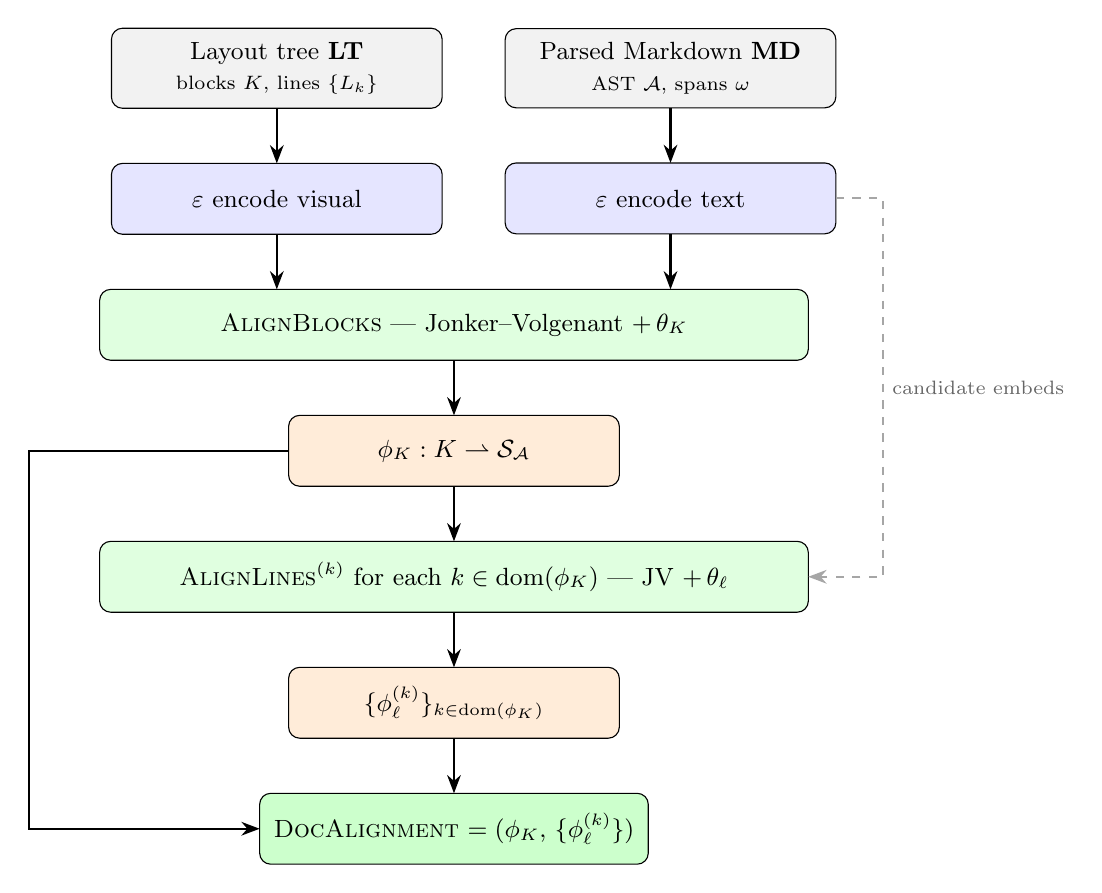
\begin{tikzpicture}[
                  box/.style={draw, rounded corners, font=\small, inner sep=5pt,
                              minimum width=4.2cm, minimum height=0.9cm, align=center},
                  input/.style={box, fill=gray!10},
                  stage/.style={box, fill=blue!10},
                  match/.style={box, fill=green!12},
                  thr/.style={box, fill=orange!15},
                  output/.style={box, fill=green!20},
                  arr/.style={->, >=Stealth, thick},
                  node distance=0.7cm and 0.8cm,
                  every node/.append style={outer sep=0pt},
            ]
            % Row 1: inputs (side-by-side)
            \node[input] (lt) {Layout tree $\LT$\\\scriptsize blocks $K$, lines $\{L_k\}$};
            \node[input, right=of lt] (md) {Parsed Markdown $\MD$\\\scriptsize AST $\mathcal{A}$, spans $\omega$};

            % Row 2: encoders
            \node[stage, below=of lt] (encv) {$\varepsilon$ encode visual};
            \node[stage, below=of md] (enct) {$\varepsilon$ encode text};

            % Row 3: block matcher (spans both columns)
            \node[match, below=of encv, xshift=2.25cm, minimum width=9cm] (bm)
            {\textsc{AlignBlocks} --- Jonker--Volgenant $+\,\theta_K$};

            % Row 4: block alignment output
            \node[thr, below=of bm] (phik)
            {$\phi_K : K \rightharpoonup \Spans_{\mathcal{A}}$};

            % Row 5: line matcher (per block)
            \node[match, below=of phik, minimum width=9cm] (lm)
            {\textsc{AlignLines}$^{(k)}$ for each $k\in\mathrm{dom}(\phi_K)$ --- JV $+\,\theta_\ell$};

            % Row 6: line alignments
            \node[thr, below=of lm] (phil) {$\{\phi_\ell^{(k)}\}_{k\in\mathrm{dom}(\phi_K)}$};

            % Row 7: output
            \node[output, below=of phil] (out) {\textsc{DocAlignment} $= (\phi_K,\, \{\phi_\ell^{(k)}\})$};

            % Arrows
            \draw[arr] (lt) -- (encv);
            \draw[arr] (md) -- (enct);
            \draw[arr] (encv) -- (bm.north -| encv);
            \draw[arr] (enct) -- (bm.north -| enct);
            \draw[arr] (bm) -- (phik);
            \draw[arr] (phik) -- (lm);
            % text-candidate embeddings reused for line matching
            \draw[arr, dashed, gray!70] (enct.east) -- ++(0.6,0)
            |- (lm.east) node[pos=0.25, right, font=\scriptsize, gray!80!black]
                  {candidate embeds};
            \draw[arr] (lm) -- (phil);
            \draw[arr] (phil) -- (out);
            % phi_K also flows to DocAlignment (side path, routed clear of AlignLines)
            \draw[arr] (phik.west) -| ([xshift=-0.9cm]lm.west) |- (out.west);

      \end{tikzpicture}
      \caption{Pipeline view of hierarchical alignment.  Visual and textual
            content are independently encoded by $\varepsilon$ (blue).
            \textsc{AlignBlocks} (green) produces the block-level partial
            mapping $\phi_K$, which conditions \textsc{AlignLines} on each
            matched block's AST-node range.  Both matchers share
            \cref{alg:match} --- Jonker--Volgenant assignment followed by
            $\theta$-thresholding (orange).  The final \textsc{DocAlignment}
            bundles $\phi_K$ and the per-block line alignments.}
      \label{fig:pipeline}
      \vspace{0.2em}
\end{figure}

%% ---------------------------------------------------------------
\section{System Implementation}
\label{sec:impl}
%% ---------------------------------------------------------------

The algorithms of \cref{sec:algo} are realized as a three-package Python
and TypeScript system: \texttt{ppx-ocr} produces per-page visual tokens
and Markdown from a raster PDF, \texttt{ppx-align} builds the layout tree,
runs embedding-based alignment, and exposes the result over HTTP, and
\texttt{ppx-svelte} is an interactive browser client that consumes the
HTTP API to display synchronized views of the page image and the
Markdown.  \cref{fig:sys-arch} gives the top-level picture.

\begin{figure}[h]
      \centering
      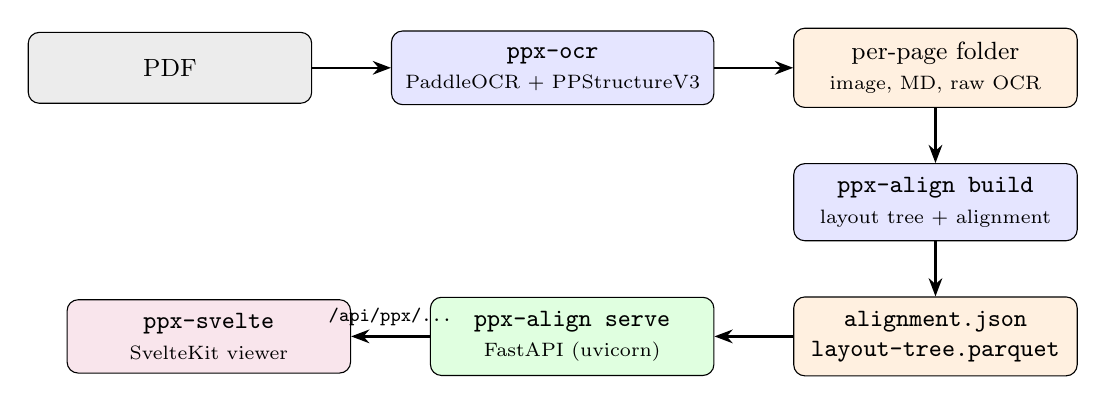
\begin{tikzpicture}[
                  box/.style={draw, rounded corners, font=\small, inner sep=5pt,
                              minimum width=3.6cm, minimum height=0.9cm, align=center},
                  pkg/.style={box, fill=blue!10},
                  svc/.style={box, fill=green!12},
                  store/.style={box, fill=orange!12},
                  client/.style={box, fill=purple!10},
                  arr/.style={->, >=Stealth, thick},
                  node distance=0.7cm and 1.0cm,
            ]
            \node[box, fill=gray!15] (pdf) {PDF};
            \node[pkg, right=of pdf] (ocr) {\texttt{ppx-ocr}\\\scriptsize PaddleOCR + PPStructureV3};
            \node[store, right=of ocr] (fs) {per-page folder\\\scriptsize image, MD, raw OCR};
            \node[pkg, below=of fs] (build) {\texttt{ppx-align build}\\\scriptsize layout tree + alignment};
            \node[store, below=of build] (aligned) {\texttt{alignment.json}\\\texttt{layout-tree.parquet}};
            \node[svc, left=of aligned] (serve) {\texttt{ppx-align serve}\\\scriptsize FastAPI (uvicorn)};
            \node[client, left=of serve] (svelte) {\texttt{ppx-svelte}\\\scriptsize SvelteKit viewer};

            \draw[arr] (pdf) -- (ocr);
            \draw[arr] (ocr) -- (fs);
            \draw[arr] (fs) -- (build);
            \draw[arr] (build) -- (aligned);
            \draw[arr] (aligned) -- (serve);
            \draw[arr] (serve) -- node[above, font=\scriptsize] {\texttt{/api/ppx/\ldots}} (svelte);

      \end{tikzpicture}
      \caption{System architecture.  Solid arrows denote data flow; orange
            nodes are on-disk artifacts.  \texttt{ppx-ocr} runs the
            PaddleOCR / PPStructure\,V3 pipeline and writes one folder per page.
            \texttt{ppx-align build} ingests those folders, constructs the
            Layout Tree and Markdown AST, and persists \texttt{alignment.json}
            and \texttt{layout-tree.parquet}.  \texttt{ppx-align serve} is a FastAPI
            backend that streams images, Markdown, tree rows, and alignments
            over JSON to the SvelteKit client.}
      \label{fig:sys-arch}
\end{figure}

\subsection{PaddleOCR and PaddlePaddle Integration}
\label{sec:paddle}

PaddleOCR is a Python OCR toolkit built on the PaddlePaddle
deep-learning framework \cite{PaddleOCR30}, and it supplies
\texttt{ppx} with the two representations the alignment pipeline
consumes.  We invoke two of its high-level APIs at complementary
granularities.  \texttt{PaddleOCR} \cite{PaddleOCRv3} is the
text-recognition entry point: given a page image it returns line-
and word-level bounding boxes together with their OCR
transcriptions.  We disable document unwarping because page
rectification has already been handled upstream by the PDF
renderer.  \texttt{PPStructureV3} \cite{PPDocLayout} is the
document-structure analyzer: it produces region- and block-level
bounding boxes labeled with semantic categories (titles,
paragraphs, tables, figures, formulas) and returns a Markdown
rendering of the page.  Both models share the PaddlePaddle runtime,
and \texttt{ppx-ocr} instantiates each exactly once per process,
caching them with \texttt{functools.cache} so that the GPU
model-load cost is paid once and amortized across every page.

Keeping the two models behind separate adapters also makes the
pipeline portable.  \texttt{ppx-ocr} constructs two intermediate
layer bundles --- \texttt{VisualTokenLayers} for the lines and words
from \texttt{PaddleOCR} and \texttt{LayoutLayers} for the regions,
blocks, and formulas from \texttt{PPStructureV3} --- and merges them
into a single \texttt{VisualLayers} dataclass consumed downstream.
The split isolates each Paddle model behind a well-typed boundary,
so a future backend change (for example to the vision-language
PaddleOCR-VL \cite{paddleocrvl2025}) touches one adapter only rather
than leaking through the rest of the pipeline.

\begin{lstlisting}[caption={Caching PaddlePaddle model instances
      (\texttt{ppx-ocr/core/ocr.py}).},
    label={lst:paddle-models}]
from functools import cache
from paddleocr import PaddleOCR, PPStructureV3

@cache
def get_ocr_model():
    return PaddleOCR(use_doc_unwarping=False)

@cache
def get_structure_model():
    return PPStructureV3()
\end{lstlisting}

\subsection{OCR and Layout Analysis Pipeline}
\label{sec:pipeline}

The \texttt{ppx-ocr} command-line driver \cite{PaddleOCR30} converts
a PDF into a directory structure keyed by page index, with one
subfolder per page containing all artifacts downstream stages need.
The canonical artifacts include the rasterized RGB page image, the
Markdown rendering produced by \texttt{PPStructureV3}, the
region- and block-level bounding-box tables with PP-DocLayout
labels \cite{PPDocLayout}, the line- and word-level OCR detection
tables, and auxiliary outputs such as figure crops, table HTML, and
LaTeX-rendered formulas when they are present on the page.
Page directories are atomic units: the driver writes into a per-page
subfolder and, by default, skips pages whose folder already exists.
The ingest stage is therefore safe to resume after a crash and
cheap to re-run incrementally as new pages are added to a
document.

\subsection{Type-Safe Data Representations}
\label{sec:types}

A recurring source of bugs in document-analysis pipelines is silent
schema drift between stages: a column rename in OCR output that
goes unnoticed until an alignment metric mysteriously drops several
weeks later.  \texttt{ppx} guards against this with two
complementary layers of validation, one for tabular artifacts and
one for structured values.

Tabular artifacts --- bounding-box tables, word tokens, layout rows
--- are declared as subclasses of \texttt{pandera.DataFrameModel}
with explicit columns, dtypes, and nullability constraints.  Schemas
such as \texttt{LineTokenSchema}, \texttt{WordTokenSchema},
\texttt{LayoutSchema}, \texttt{BlockSchema}, and
\texttt{LayoutTreeSchema} are validated at every stage boundary, so
a type mismatch between \texttt{ppx-ocr} output and
\texttt{ppx-align} input surfaces as a structured Pandera error
rather than as a silent numerical regression downstream.

Non-tabular values --- \texttt{ParsedDocument},
\texttt{BlockAlignmentTarget}, \texttt{CharAlignmentTarget},
\texttt{DocAlignment} --- are Pydantic \texttt{BaseModel}s.  The
alignment results in particular are wire-format-ready:
\texttt{DocAlignment} serializes directly to the JSON consumed by
the HTTP API (\cref{sec:clientserver}), closing the loop from
algorithmic output to network response with no ad-hoc marshaling
code.

\begin{lstlisting}[caption={Pydantic models for alignment targets
      (\texttt{ppx-align/core/types.py}).},
    label={lst:align-types}]
class BlockAlignmentTarget(BaseModel):
    ast_start: int
    ast_end: int
    score: float

class CharAlignmentTarget(BaseModel):
    ast_index_start: int
    char_start: int
    ast_index_end: int
    char_end: int
    score: float

class DocAlignment(BaseModel):
    block_alignments: dict[str, BlockAlignmentTarget]
    line_alignments:  dict[str, CharAlignmentTarget]
\end{lstlisting}

\subsection{Composable Pipeline Design}
\label{sec:compose-sys}

Every stage of the pipeline --- OCR, structure analysis,
layout-tree construction, Markdown parsing, block alignment, line
alignment --- is a pure function from one validated artifact to
another.  The types of \cref{sec:types} are the glue that makes
this composition safe: a stage advertises its input and output as
Pandera or Pydantic types, and a mismatched upstream raises at the
boundary rather than silently corrupting downstream results.
Representative signatures include
\texttt{build\_parsed\_doc(MarkdownDocument) -> ParsedDocument} for
the Markdown side, \texttt{align\_blocks} returning a mapping from
block node ids to \texttt{BlockAlignmentTarget}, and
\texttt{align\_tree} returning the full \texttt{DocAlignment} that
the server consumes.  No stage mutates its inputs; each returns a
new artifact that can be cached, persisted, or fed to multiple
downstream stages.  The \texttt{ppx-align} encoder runs the
\texttt{SentenceTransformer} forward pass on a CUDA device when one
is available, with a CPU fallback preserved for development.

The Markdown side of the pipeline deserves particular attention
because it bridges the OCR output and the AST indices the
formulation of \cref{sec:formal} is built on.
\texttt{build\_parsed\_doc} (in \texttt{ppx-align/core/md.py})
parses the OCR-generated Markdown with \texttt{markdown-it-py} in
GFM-like mode, extracts the top-level syntax-tree children as the
AST leaf sequence $\mathcal{A}$, and derives character spans
$\sigma$ from the \texttt{node.map} line indices combined with an
offset table computed from \texttt{splitlines(keepends=True)}.  Word
spans $\omega$ are produced by NLTK's
\texttt{TreebankWordTokenizer.span\_tokenize} applied to each AST
node's content.  A single helper function,
\texttt{get\_content}, dispatches over an AST range, an AST index,
a \texttt{BlockAlignmentTarget}, or a \texttt{CharAlignmentTarget}
to recover the Markdown slice backing any alignment artifact,
giving viewers and debuggers a uniform retrieval API without
re-implementing span arithmetic.

The \texttt{ppx-align} CLI orchestrates these stage functions in
dependency order and writes \texttt{layout-tree.parquet} and
\texttt{alignment.json} into each page directory.  It supports
common partial-execution modes --- single-page runs, a
blocks-only mode, and the noise-variant benchmark runs used in
\cref{sec:bench} --- through optional flags; we refer the reader to
the project repository for the full command-line surface.  The
benchmark-variant runs are worth naming explicitly because they are
how \cref{sec:bench}'s results come into being: a single invocation
can produce auxiliary artifacts named \texttt{markdown\_\{level\}.md}
and \texttt{alignment\_\{level\}.json} alongside the canonical
artifacts, one pair per noise level, which \texttt{ppx-bench}
later consumes directly without re-running the OCR stage.

\subsection{Client/Server Architecture for AI-Assisted Reading}
\label{sec:clientserver}

The alignment artifacts are only useful if a human --- or an LLM
agent --- can explore them.  To that end, \texttt{ppx-align serve}
exposes a thin FastAPI facade over the on-disk output directory,
and \texttt{ppx-svelte} consumes it in the browser.  The backend
streams JSON endpoints for document listing, per-page page images
and thumbnails, the raw and parsed Markdown, the layout tree rows,
and the \texttt{DocAlignment} itself; the viewer is a SvelteKit /
Vite application that reaches the backend through the Vite dev
proxy in development and a reverse proxy in production.  The
project repository is the authoritative reference for the exact
route surface.

The viewer renders a two-panel layout --- page image on the left,
Markdown on the right --- and fetches each document's tree and
alignment lazily on page change.  Hovering a visual-token overlay
highlights the aligned Markdown span and scrolls the right panel to
it; toggling \emph{Raw} exposes the Markdown source for reverse
selection, in which case the selected character range is displayed
as an \texttt{ast\_index:char\_offset} span that can be copied into
downstream tooling.  \Cref{fig:viewer-thumbs} shows the viewer in
use on two documents from the benchmark corpus, with full-size
versions collected in \cref{app:viewer-full}
(\cref{fig:viewer-clip-full,fig:viewer-resnet-full}).  The left panel
of each screenshot renders the original source PDF with the hovered
visual token's bounding box highlighted, while the right panel shows
the corresponding span in the raw OCR-generated Markdown.  Both
examples expose real OCR artifacts --- collapsed table structure in
the CLIP example, raw \texttt{\$\ldots\$} equation delimiters in the
ResNet example --- yet the alignment still resolves to the correct
span, which is consistent with the content-type resilience
quantified in \cref{sec:bench-vanilla}.

Separating \texttt{build} from \texttt{serve} is a deliberate
architectural choice.  Alignment is GPU-heavy and batch-oriented;
serving is I/O bound and latency-sensitive.  Splitting them lets
the heavy stage run once per corpus update --- producing the typed
artifacts the server then reads directly --- while the server runs
as a lightweight sidecar.  The server deliberately has no model
dependencies (no PaddlePaddle, no PyTorch), which keeps its
container footprint small and lets it be deployed behind an
authenticating reverse proxy without exposing the model runtime or
its GPU weights to the network.

\begin{figure}[h]
      \centering
      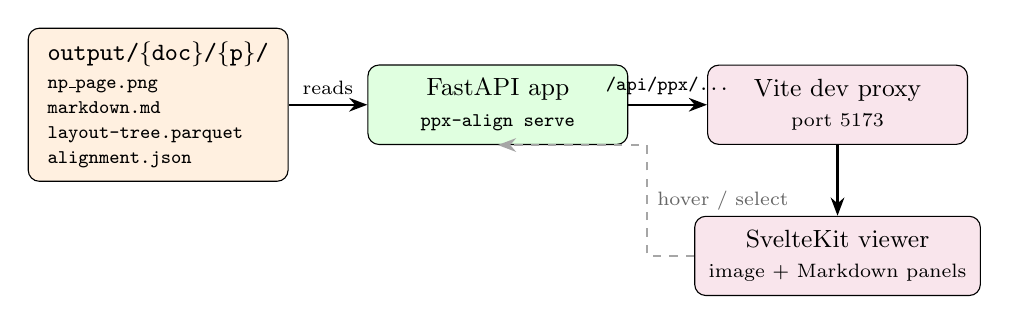
\begin{tikzpicture}[
                  box/.style={draw, rounded corners, font=\small, inner sep=5pt,
                              minimum width=3.3cm, minimum height=0.9cm, align=center},
                  svr/.style={box, fill=green!12},
                  cli/.style={box, fill=purple!10},
                  disk/.style={box, fill=orange!12},
                  arr/.style={->, >=Stealth, thick},
                  node distance=0.9cm and 1.0cm,
            ]
            \node[disk, align=left] (out) {\texttt{output/\{doc\}/\{p\}/}\\[-1pt]
                  \scriptsize\texttt{np\_page.png}\\[-2pt]
                  \scriptsize\texttt{markdown.md}\\[-2pt]
                  \scriptsize\texttt{layout-tree.parquet}\\[-2pt]
                  \scriptsize\texttt{alignment.json}};
            \node[svr, right=of out] (api) {FastAPI app\\\scriptsize
                  \texttt{ppx-align serve}};
            \node[cli, right=of api] (vite) {Vite dev proxy\\\scriptsize port 5173};
            \node[cli, below=of vite] (ui) {SvelteKit viewer\\\scriptsize
                  image + Markdown panels};

            \draw[arr] (out) -- node[above, font=\scriptsize] {reads} (api);
            \draw[arr] (api) -- node[above, font=\scriptsize]
            {\texttt{/api/ppx/\ldots}} (vite);
            \draw[arr] (vite) -- (ui);
            \draw[arr, dashed, gray!70] (ui.west) -- ++(-0.6,0) |-
            node[pos=0.25, right, font=\scriptsize, gray!80!black]
                  {hover / select} (api.south);
      \end{tikzpicture}
      \caption{Client/server topology.  \texttt{ppx-align serve} reads
            per-page artifacts from disk and exposes them as JSON and static
            resources.  The SvelteKit viewer reaches the backend through the
            Vite dev proxy in development and a reverse proxy in production.
            The dashed arrow denotes user interactions (hover highlights,
            reverse text selection) that issue additional API requests.}
      \label{fig:clientserver}
\end{figure}

\begin{figure}[h]
      \centering
      \begin{minipage}{0.48\linewidth}
            \centering
            \hyperref[fig:viewer-clip-full]{%
                  
\includegraphics[width=\linewidth]{notes/ppx-svelte-img-4.png}}
      \end{minipage}\hfill
      \begin{minipage}{0.48\linewidth}
            \centering
            \hyperref[fig:viewer-resnet-full]{%
                  
\includegraphics[width=\linewidth]{notes/ppx-svelte-img-5.png}}
      \end{minipage}
      \caption{Thumbnails of \texttt{ppx-svelte} viewing the CLIP
            paper (left) and the ResNet paper (right).  In each
            screenshot the left-hand panel of the viewer shows the
            original source PDF with the hovered visual token's
            bounding box highlighted, and the right-hand panel shows
            the corresponding span in the raw OCR-generated Markdown.
            OCR artifacts --- collapsed tables in the CLIP example,
            raw \texttt{\$\ldots\$} equation delimiters in the ResNet
            example --- are preserved intentionally: the alignment
            resolves to the correct span regardless of downstream
            text quality.  Click either thumbnail in an interactive
            PDF viewer to jump to the full-size version in
            \cref{app:viewer-full} (\cref{fig:viewer-clip-full,fig:viewer-resnet-full}).}
      \label{fig:viewer-thumbs}
\end{figure}

\FloatBarrier

%% ---------------------------------------------------------------
\section{Benchmark}
\label{sec:bench}
%% ---------------------------------------------------------------

We quantify the pipeline's behavior along three axes: alignment quality
on uncorrupted inputs, degradation under controlled OCR-noise injection,
and precision / recall / F1 relative to the uncorrupted reference.  All
experiments are implemented in the \texttt{ppx-bench} package.

\subsection{Setup}
\label{sec:bench-setup}

\paragraph{Corpus.}
We run the benchmarks over a corpus of six academic documents ---
\texttt{PubLayNet}, \texttt{clip}, \texttt{deeplearning},
\texttt{paddleocrv3}, \texttt{resnet}, and \texttt{rl} --- spanning
130 pages after processing through the \texttt{ppx-ocr} and
\texttt{ppx-align} pipeline of \cref{sec:impl}.  Together the corpus
yields 1{,}505 block-level visual tokens and 13{,}908 line-level visual
tokens, a scale sufficient to expose both aggregate trends and
per-label subpopulations.  The per-document composition is summarized
in \cref{tab:bench-corpus}.

The six documents were selected as a convenience sample spanning
several machine-learning subdomains (layout analysis, vision--language,
vision, reinforcement learning, and a technical report), with a bias
toward well-known papers whose OCR output we could sanity-check by
reading.  The sample is not intended as a representative corpus and
its small size is an acknowledged limitation; the primary purpose is
to exercise the pipeline across varied page structures.

\begin{table}[h]
      \centering
      \small
      \begin{tabular}{lrrr}
            \toprule
                           & \textbf{pages} & \textbf{blocks}  & \textbf{lines}    \\
            \midrule
            PubLayNet      & 8              & 95               & 891               \\
            clip           & 48             & 536              & 5{,}062           \\
            deeplearning   & 10             & 114              & 1{,}076           \\
            paddleocrv3    & 24             & 270              & 2{,}459           \\
            resnet         & 12             & 148              & 1{,}340           \\
            rl             & 28             & 342              & 3{,}080           \\
            \midrule
            \textbf{total} & \textbf{130}   & \textbf{1{,}505} & \textbf{13{,}908} \\
            \bottomrule
      \end{tabular}
      \caption{Benchmark corpus composition.  All six documents are
            academic papers with the exception of \texttt{paddleocrv3},
            which is a technical report.  Block and line counts are the
            totals reported by \texttt{ppx-align} after building the
            Layout Tree for each page.}
      \label{tab:bench-corpus}
\end{table}

\paragraph{Block-label distribution.}
The PP-DocLayout categories assigned to each block determine which
parent-label bucket each line inherits, and --- as \cref{sec:bench-vanilla}
shows --- are the strongest predictor of alignment quality.
\cref{tab:bench-labels} lists the distribution; \texttt{text},
\texttt{paragraph\_title}, \texttt{figure\_title}, and \texttt{number}
dominate, with a long tail of formula-, table-, and image-type blocks.
The 541 lines carrying the sentinel \texttt{unknown} parent label
correspond to structural gaps in the OCR output where a line was
detected but not assigned to any block.

\begin{table}[h]
      \centering
      \small
      \begin{tabular}{lrrrr}
            \toprule
            \textbf{label}                & \textbf{blocks} & \textbf{block mean} & \textbf{lines} & \textbf{line mean} \\
            \midrule
            text                          & 718             & 0.97                & 5{,}114        & 0.96               \\
            paragraph\_title              & 144             & 0.82                & 149            & 0.96               \\
            figure\_title                 & 119             & 0.80                & 492            & 0.97               \\
            number                        & 118             & 0.02                & 1              & 0.00               \\
            header                        & 77              & 0.39                & 64             & 0.55               \\
            formula                       & 62              & 0.98                & 268            & 0.75               \\
            formula\_number               & 55              & 0.18                & 1              & 0.00               \\
            table                         & 43              & 0.90                & 2{,}035        & 0.99               \\
            image                         & 37              & 0.37                & 1{,}291        & 0.42               \\
            reference                     & 31              & 1.00                & 1{,}416        & 0.96               \\
            chart                         & 30              & 0.41                & 2{,}137        & 0.45               \\
            footer                        & 26              & 0.02                & 26             & 0.02               \\
            footnote                      & 14              & 0.45                & 43             & 0.52               \\
            algorithm                     & 8               & 1.00                & 204            & 0.95               \\
            aside\_text                   & 8               & 0.32                & 14             & 0.58               \\
            abstract                      & 6               & 1.00                & 99             & 0.96               \\
            doc\_title                    & 5               & 0.90                & 6              & 1.00               \\
            vision\_footnote              & 3               & 1.00                & 3              & 1.00               \\
            reference\_content            & 1               & 0.00                & 4              & 0.00               \\
            \texttt{unknown} (lines only) & ---             & ---                 & 541            & 0.00               \\
            \bottomrule
      \end{tabular}
      \caption{Block-label distribution across the corpus, together with
            the mean alignment score of each label at block and line
            granularity.  Line counts exceed block counts for \texttt{text},
            \texttt{table}, \texttt{reference}, \texttt{image}, and
            \texttt{chart} because those blocks contain multiple OCR line
            tokens.}
      \label{tab:bench-labels}
\end{table}

\paragraph{Three benchmark suites.}
We report three complementary studies, each implemented as a separate
entry point in \texttt{ppx-bench}.  The \emph{vanilla} benchmark
(\cref{sec:bench-vanilla}) measures alignment-score distributions at
block and line granularity on the uncorrupted corpus; it establishes
the baseline and exposes the strong label-dependent structure of
alignment quality.  The \emph{noise} benchmark
(\cref{sec:bench-noise}) re-runs the alignment pipeline on Markdown
perturbed at corruption fractions
$\{0.00, 0.01, 0.02, 0.04, 0.05, 0.20\}$ and tracks the resulting
shift in mean line score.  The \emph{precision/recall} benchmark
(\cref{sec:bench-pr}) treats the noise-$0$ alignment as a gold-standard
proxy and computes per-line precision, recall, and $F1$ at 13 noise
levels densely sampled in $[0, 0.2]$, isolating the transition from
intact behavior to catastrophic failure.

\paragraph{Corruption model.}
The corruption routine in \texttt{ppx-bench.core.corrupt} operates on
the Markdown string directly.  For each line alignment target, it
recovers the line's absolute character span and replaces a
\texttt{noise\_level} fraction of those characters with a random draw
from
$\texttt{ascii\_letters} \cup \texttt{digits} \cup \texttt{punctuation} \cup \{\texttt{space}\}$.
Characters outside any line span --- structural Markdown such as
heading markers, blank lines, HTML table markup --- are preserved, so
corruption affects only the portions of the document the aligner
actually consumes.  Overlapping spans are de-duplicated to prevent
double-corruption of shared characters.  By operating per span rather
than uniformly over the Markdown, the corruption rate seen by each
aligned line matches \texttt{noise\_level} in expectation, and
propagates proportionally to the block level (each block being a union
of its line spans).

\paragraph{Per-line precision and recall.}
For each line $\ell$ with a gold-standard alignment, we first check
whether the parent block's AST-node range agrees between the gold and
noisy alignments.  If it does not, we classify $\ell$ as a
\emph{block error} and record $(P, R) = (0, 0)$: the line cannot
possibly land correctly because its containing block has been
reassigned.  When the parent block matches, we compute absolute
character spans $[g_s, g_e)$ and $[n_s, n_e)$ for the gold and noisy
alignments in each document's own Markdown coordinate system
(corruption can shift AST boundaries when structural characters
change), and set
\[
      P = \frac{|[g_s, g_e) \cap [n_s, n_e)|}{|[n_s, n_e)|},
      \qquad
      R = \frac{|[g_s, g_e) \cap [n_s, n_e)|}{|[g_s, g_e)|},
      \qquad
      F1 = \frac{2PR}{P + R}.
\]
Lines without a gold alignment are excluded from evaluation; lines
with a gold alignment but no noisy alignment are counted as $(0, 0)$.
All aggregates reported below are unweighted means over the evaluated
lines.

\subsection{Vanilla Alignment Quality}
\label{sec:bench-vanilla}

\paragraph{Aggregate scores.}
On the uncorrupted corpus, the alignment pipeline achieves a mean block
overlap of $0.79$ with a cross-document standard deviation of $0.07$,
and a mean line overlap of $0.80$ with $\sigma = 0.08$
(\cref{tab:bench-vanilla-agg}).  The small cross-document spread across
six structurally diverse sources indicates that the pipeline
generalizes: no single document pulls the aggregate in either
direction.

\begin{table}[h]
      \centering
      \small
      \begin{tabular}{lrr}
            \toprule
                   & \textbf{mean} & \textbf{cross-doc $\sigma$} \\
            \midrule
            Blocks & 0.79          & 0.07                        \\
            Lines  & 0.80          & 0.08                        \\
            \bottomrule
      \end{tabular}
      \caption{Aggregate alignment-score statistics on the uncorrupted
            corpus.  Means are computed over all 1{,}505 blocks and 13{,}908
            lines; $\sigma$ is across the six documents.}
      \label{tab:bench-vanilla-agg}
\end{table}

The per-document kernel-density estimates of line score all share a
single peak near $\mathrm{score} = 1.0$, with \texttt{rl} the one
visibly flatter curve; the remaining five documents track one another
closely.

\paragraph{Structural bimodality by block label.}
The aggregate hides substantial structural variation.  Grouping by
block label reveals a strong bimodal split between \emph{text-like}
content, which aligns near-perfectly, and \emph{non-textual or
      sparse-signal} content, which aligns poorly or not at all.
\cref{tab:bench-vanilla-bimodality} summarizes the groups.

\begin{table}[h]
      \centering
      \small
      \begin{tabular}{@{}p{4.3cm}cp{6.3cm}@{}}
            \toprule
            \textbf{label group}                      & \textbf{line mean} & \textbf{interpretation} \\
            \midrule
            \texttt{text}, \texttt{paragraph\_title},
            \texttt{table}, \texttt{reference},
            \texttt{figure\_title}, \texttt{algorithm},
            \texttt{abstract}                         & 0.95--0.99         &
            text-like content aligns near-perfectly                                                  \\[2pt]
            \texttt{formula}                          & 0.75               &
            block matches well (block mean $0.98$) but character
            spans inside the formula only partially overlap Markdown
            nodes                                                                                    \\[2pt]
            \texttt{chart}, \texttt{image}            & 0.45,\ 0.42        &
            non-textual OCR content has no semantic anchor in the
            Markdown stream                                                                          \\[2pt]
            \texttt{header}                           & 0.55               &
            running heads are repetitive across pages; distinctive
            tokens keep individual lines alignable even though the
            block-level score (block mean $0.39$) is low                                             \\[2pt]
            \texttt{footer}                           & 0.02               &
            page numbers and short footers; low-signal for sentence
            embeddings                                                                               \\[2pt]
            \texttt{unknown}                          & 0.00               &
            541 lines with no block label; a structural gap in the
            OCR output                                                                               \\[2pt]
            \texttt{formula\_number}, \texttt{number} &
            --- ($n{=}1$ each, trivial)               &
            short numeric content fails at the block level (block
            means $0.18$ / $0.02$); nearly no lines assigned at the
            line level                                                                               \\
            \bottomrule
      \end{tabular}
      \caption{Line-level mean alignment score by block-label group.
            Values in the middle column are \emph{line means}; block-level
            context is given in-row where it clarifies the behavior.
            Text-like content and non-textual content sit on opposite
            ends of the distribution, with almost no mass in the
            middle.}
      \label{tab:bench-vanilla-bimodality}
\end{table}

The stacked histogram of \cref{fig:bench-vanilla-stacked} makes the
bimodality concrete.  Mass at $\mathrm{score} = 1.0$ is almost
entirely contributed by \texttt{text}, \texttt{table}, and
\texttt{reference} lines; mass at $\mathrm{score} = 0$ is
\texttt{unknown} and \texttt{image}.  The middle of the range is
largely empty.

\paragraph{Interpretation.}
Alignment quality is a function of content type rather than a uniform
``good/bad'' attribute of the pipeline.  The gap between the aggregate
($0.80$) and a hypothetical ceiling of $1.0$ is driven almost entirely
by the $20$--$30\%$ of lines whose block label is
\texttt{image}, \texttt{chart}, \texttt{number}, \texttt{header}, or
\texttt{footer} --- categories for which the OCR transcription carries
little to no semantic content that an embedding-based matcher could
anchor to.  We interpret this as a fundamental property of the
formulation (cosine similarity of Sentence-BERT embeddings requires
semantic content on both sides) rather than a regression that further
algorithmic tuning could close.

\paragraph{Per-document outliers.}
\texttt{rl} sits meaningfully below the rest of the corpus with a
line-level mean of $0.64$.  Inspection reveals dense figure content
and short, symbol-heavy labels, both of which push more of its lines
into the low-mean label groups above.  \texttt{PubLayNet} and
\texttt{resnet} lead the corpus at approximately $0.88$, reflecting
longer, text-heavy paragraphs with few auxiliary blocks.

\begin{figure}[h]
      \centering
      
\includegraphics[width=0.75\linewidth]{../../output/benchmark/line_combined.png}
      \caption{Uncorrupted line-score histogram stacked by block label.
            Mass at $\mathrm{score}{=}1.0$ is almost entirely
            \texttt{text} / \texttt{table} / \texttt{reference}; mass at
            $\mathrm{score}{=}0$ is \texttt{unknown} plus \texttt{image}.
            Structural bimodality across content types is concrete rather than
            a tail artifact.}
      \label{fig:bench-vanilla-stacked}
\end{figure}

\subsection{Noise Robustness}
\label{sec:bench-noise}

\paragraph{Score degradation with noise.}
Injecting character-level corruption into each line's Markdown span
causes the mean line-level alignment score to fall with the
corruption fraction, but the fall is not strictly monotone near the
origin.  \cref{tab:bench-noise} lists the 13 sampled levels along
with the corresponding mean line scores and relative drops from
baseline.  At noise $0.005$ the mean score actually \emph{rises} by
$0.6\%$; between $0.005$ and $0.007$ it barely moves.  This
apparent stability is misleading, as we explain below: the
line-score metric measures how well a line matches \emph{wherever}
it ended up, not whether it ended up in the right place, and by
the time the score begins its sustained decline the block-error
rate of \cref{sec:bench-pr} has already tripled.  From noise
$0.009$ onward the descent is cleanly monotone, ending at $0.469$
at noise $0.20$ --- a $40.5\%$ drop from baseline.

\begin{table}[h]
      \centering
      \small
      \begin{tabular}{rrr}
            \toprule
            \textbf{noise} & \textbf{mean line score} & \textbf{drop from baseline} \\
            \midrule
            0.000          & 0.787                    & ---                         \\
            0.005          & 0.792                    & $+0.6\%$                    \\
            0.006          & 0.782                    & $-0.6\%$                    \\
            0.007          & 0.784                    & $-0.4\%$                    \\
            0.008          & 0.774                    & $-1.7\%$                    \\
            0.009          & 0.760                    & $-3.5\%$                    \\
            0.010          & 0.750                    & $-4.8\%$                    \\
            0.020          & 0.734                    & $-6.8\%$                    \\
            0.030          & 0.702                    & $-10.8\%$                   \\
            0.040          & 0.690                    & $-12.4\%$                   \\
            0.050          & 0.669                    & $-15.0\%$                   \\
            0.100          & 0.590                    & $-25.1\%$                   \\
            0.200          & 0.469                    & $-40.5\%$                   \\
            \bottomrule
      \end{tabular}
      \caption{Mean line-level alignment score across the 13 noise
            levels sampled by the noise benchmark.  Degradation is
            monotonic \emph{in the large} but the line-score metric
            is indifferent to whether a line ended up in its correct
            block: at noise $0.005$--$0.007$ the score barely changes
            (and slightly \emph{rises} at $0.005$), while the
            block-error rate reported in \cref{sec:bench-pr} has
            already begun to climb.}
      \label{tab:bench-noise}
\end{table}

\paragraph{Distributional shift.}
\cref{fig:bench-noise} visualizes the same data as per-noise kernel
density estimates.  The score-$1.0$ peak visible at noise $0$
progressively shifts leftward and flattens as corruption grows, with
probability mass moving from the unit-peak toward the middle of the
range.  The shape of the shift is consistent with a gradual
deterioration of individual matches rather than a single catastrophic
drop at a critical noise level --- a picture that the denser sampling
of \cref{sec:bench-pr} will refine into a staircase.

\paragraph{Parallel per-document trajectories.}
All six documents share the same decay slope.  \texttt{PubLayNet} and
\texttt{resnet} --- the strongest baselines --- remain on top at every
noise level ($0.89 \to 0.49$ and $0.88 \to 0.58$ between noise $0$ and
$0.20$).  \texttt{rl} remains at the bottom ($0.64 \to 0.45$).  No
document ``breaks'' catastrophically before others; the per-document
ordering at noise $0$ is preserved throughout the sampled range.
Cross-document differences are expressed as a vertical offset on the
score axis rather than as differential sensitivity to noise.

\begin{figure}[h]
      \centering
      
\includegraphics[width=0.75\linewidth]{../../output/noise_benchmark/line_overlap.png}
      \caption{Per-noise KDE of line scores.  Each curve is the
            distribution at one corruption level; the score-$1.0$ peak
            progressively shifts leftward and flattens as noise increases,
            with mass moving from the unit-peak toward the middle of the
            range.}
      \label{fig:bench-noise}
\end{figure}

\subsection{Precision, Recall, and F1 under Noise}
\label{sec:bench-pr}

\paragraph{Headline results.}
Densely sampling noise levels in $[0, 0.2]$ and computing
precision / recall / F1 against the noise-$0$ alignment resolves the
smooth curve of \cref{sec:bench-noise} into a \emph{staircase} with
two discrete step-changes and an earlier shoulder.
\cref{tab:bench-pr} reports the 13-point sweep.

\begin{table}[h]
      \centering
      \small
      \begin{tabular}{rrrrrl}
            \toprule
            \textbf{noise} & \textbf{P} & \textbf{R} & \textbf{F1} & \textbf{block err} & \textbf{regime}     \\
            \midrule
            0.000          & 1.00       & 1.00       & 1.00        & 0\%                & intact              \\
            0.005          & 0.90       & 0.90       & 0.90        & 3\%                & early shoulder      \\
            0.006          & 0.85       & 0.85       & 0.85        & 10\%               & block-error triples \\
            0.007          & 0.83       & 0.82       & 0.82        & 12\%               & smooth              \\
            0.008          & 0.81       & 0.81       & 0.81        & 11\%               & smooth              \\
            0.009          & 0.73       & 0.72       & 0.72        & 18\%               & \textbf{step \#1}   \\
            0.01           & 0.70       & 0.68       & 0.68        & 22\%               & smooth              \\
            0.02           & 0.64       & 0.61       & 0.62        & 26\%               & smooth              \\
            0.03           & 0.53       & 0.50       & 0.51        & 36\%               & \textbf{step \#2}   \\
            0.04           & 0.50       & 0.46       & 0.47        & 39\%               & smooth              \\
            0.05           & 0.45       & 0.41       & 0.42        & 41\%               & smooth              \\
            0.10           & 0.32       & 0.29       & 0.29        & 48\%               & tail                \\
            0.20           & 0.14       & 0.12       & 0.13        & 64\%               & tail                \\
            \bottomrule
      \end{tabular}
      \caption{Mean precision, recall, $F1$, and block-error rate at each
            of the 13 sampled noise levels.  Block-error rate is the fraction
            of lines whose parent block is reassigned under corruption, each
            of which contributes $(P, R) = (0, 0)$ to the averages.}
      \label{tab:bench-pr}
\end{table}

\cref{fig:bench-pr-line} plots the same data against a continuous
noise axis.  The staircase structure --- otherwise invisible in the
smooth summary of \cref{sec:bench-noise} --- appears as visible bends
in the descent.

\paragraph{Staircase degradation.}
Between the transitions, each metric decays gently; at the steps, a
discrete cohort of blocks flips in a single doubling of the noise
level.  Step \#1, between noise $0.008$ and $0.009$, is sharp: $F1$
drops from $0.81$ to $0.72$ and the block-error rate jumps from
$11\%$ to $18\%$.  Step \#2, between $0.02$ and $0.03$, is of
comparable magnitude: $F1$ from $0.62$ to $0.51$, block-error from
$26\%$ to $36\%$.  An earlier shoulder between $0.005$ and $0.006$
triples the block-error rate ($3\% \to 10\%$) even though $F1$ moves
by only $0.05$ --- the damage registers first on blocks and only
later propagates into line-level scores.  We hypothesize that the
staircase reflects content-length variation in block embeddings:
short, low-distinctiveness blocks lose their similarity margin earlier
than long, text-rich blocks, so increasing noise knocks out successive
cohorts at distinct thresholds.  Validating this mechanism per label
group is left to future work.

\paragraph{Document-specific thresholds.}
Drilling into the transition zone exposes heterogeneity across
documents.  At noise $0.006$, \texttt{paddleocrv3} and \texttt{rl}
have already crossed $25\%$ block-error, whereas \texttt{PubLayNet},
\texttt{resnet}, \texttt{clip}, and \texttt{deeplearning} remain
below $10\%$ through noise $0.008$ and only step up at $0.009$.  The
aggregate step observed at $0.009$ is thus the average of documents
that have already crossed their own first step and documents that
cross it here; per-document staircases are sharper and shifted along
the noise axis.  Weaker-baseline documents cross the first step at
lower noise, consistent with --- though not a direct proof of --- the
content-distinctiveness hypothesis above.

\paragraph{Precision, recall, and $F1$ move together.}
At every sampled noise level the three metrics stay within $0.03$ of
each other (\cref{tab:bench-pr}).  This reflects the symmetry of the
character-span overlap metric combined with the fact that when a line
matches within its correct block, the matched span is almost always
exact --- partial-overlap cases contributing asymmetric numerator and
denominator are rare.

\paragraph{Bimodal precision distribution.}
\cref{fig:bench-precision-dist} shows the per-noise distribution of
line-level precision.  At every noise level the distribution has two
peaks, near $0$ and near $1$.  Increasing noise does not smear the
middle of the range; it shifts mass from the $1$-peak to the $0$-peak.
Alignment therefore behaves as a \emph{binary} outcome per line ---
either fully correct or fully wrong --- with very little partial credit.

\paragraph{Cross-document variance peaks in the transition zone.}
Cross-document $\sigma$ on $F1$ is near zero at noise $0$ (by
definition), rises to approximately $0.08$ at noise $0.005$, widens to
$0.10$--$0.14$ across $0.02$--$0.05$, and shrinks back to $\sim 0.04$
at $0.20$.  Documents diverge most in the middle of the descent
because content-specific resilience is most visible there; at the
extremes all documents are either intact or largely broken, and
variance collapses.

\begin{figure}[h]
      \centering
      
\includegraphics[width=0.85\linewidth]{../../output/precision_recall_benchmark/pr_mean_vs_noise_line.png}
      \caption{Mean precision, recall, $F1$, and block-error rate
            plotted against a continuous noise axis with cross-document
            $\sigma$ envelopes.  The staircase structure appears as
            visible bends in the otherwise-smooth descents around noise
            $0.009$ and $0.03$.}
      \label{fig:bench-pr-line}
\end{figure}

\begin{figure}[h]
      \centering
      
\includegraphics[width=0.75\linewidth]{../../output/precision_recall_benchmark/precision_overlap.png}
      \caption{Per-noise precision distribution.  Every curve is bimodal
            with peaks near $0$ and $1$ at every noise level; increasing noise
            shifts mass \emph{between} the two peaks rather than smearing the
            middle of the range.}
      \label{fig:bench-precision-dist}
\end{figure}

\subsection{Cross-Cutting Observations}
\label{sec:bench-cross}

Taken together, the three benchmark suites expose five properties of
the pipeline that matter for downstream use and that motivate the
limitations and future-work directions of \cref{sec:conclusion}.

\paragraph{Alignment is binary per line, gated by block-level
      correctness.}  The bimodal precision distribution of
\cref{fig:bench-precision-dist}, together with the block-error rule
built into the metric, implies that line-level success depends almost
entirely on whether the parent block is correctly matched.  When the
parent block lands in the right AST-node range, the line's
character-level span is usually exact; when it does not, the line
contributes $0$ to every aggregate regardless of whether the local
matcher would have produced a reasonable span.  There is little
partial-credit behavior in between.

\paragraph{Block matching is the fragile link.}  Consequently the
block-alignment stage of \cref{sec:block} is where noise causes the
pipeline to fail.  Embedding-based block matching flips when a small
number of distinguishing tokens change, and the flip cascades into
line-level failure even though line-level matching (when it runs at
all) remains accurate.  This observation motivates both the per-label
failure analysis and the block-alignment diagnostics listed under
Future Work.

\paragraph{Non-textual content is a structural blind spot.}
\cref{tab:bench-vanilla-bimodality} shows that \texttt{image},
\texttt{chart}, \texttt{number}, \texttt{header}, and \texttt{footer}
blocks score poorly at noise $0$ and cannot be repaired by any
improvement to the alignment algorithm --- their OCR content is not a
semantic handle the Markdown provides.  This is a property of the
problem formulation, not of the pipeline, and any downstream system
that requires coverage of these categories must supply an auxiliary
matching strategy.

\paragraph{Uniform degradation across documents.}  All six documents
share the same decay trajectory under noise.  Differences between
\texttt{rl} and \texttt{PubLayNet} are expressed as a vertical offset
on the score axis rather than as differential sensitivity; the
per-document ordering at noise $0$ is preserved throughout the sampled
range.  Document-level generalization is therefore robust, even as
per-document staircases differ in where along the noise axis their
step-changes land.

\paragraph{Block-error rate is the earliest-warning metric.}  At
noise $0.005$ the mean line score actually \emph{rises} by $0.6\%$
(to $0.792$), and at noise $0.006$ it has fallen only to $0.782$ ---
a $0.6\%$ drop from baseline.  In the same range the block-error
rate triples from $3\%$ to $10\%$ and precision drops from $0.90$
to $0.85$.  Monitoring line-level scores alone would therefore
understate early-stage degradation by a wide margin; operational
deployments should treat block-error rate as the primary health
metric and line score as a secondary signal.

\FloatBarrier

%% ---------------------------------------------------------------
\section{Conclusion}
\label{sec:conclusion}
%% ---------------------------------------------------------------

This thesis set out to address the weakest rung on the agentic
knowledge-distillation ladder of \cref{sec:intro}: the correspondence
between a document and the Markdown produced from it.  We introduced
the \emph{Parsed Page eXplorer} (\texttt{ppx}) as a foundational tool
for that correspondence, developed it across three chapters, and
evaluated it on a modest but diverse benchmark.  The remainder of
this section summarizes what was contributed, what the contributions
do not resolve, and the directions for which the present work lays
the groundwork.

\subsection{Summary of Contributions}

The thesis made three contributions, each spanning one of the
paper's core chapters.  First, \cref{sec:formal} gave a
\textbf{set-theoretic formulation} of multimodal document alignment
that cleanly separates the four-level Layout Tree from the Markdown
AST and casts alignment as a pair of partial injective functions
(one at block granularity, one at line granularity) scored by
semantic similarity.  The formulation's value is not only as a
precise statement of what \texttt{ppx} computes but also as a shared
vocabulary that future systems --- whether decomposed pipelines or
integrated end-to-end models --- can use to describe their own
outputs in terms compatible with ours.

Second, \cref{sec:algo,sec:impl} presented a \textbf{composable
      pipeline} that realizes the formulation.  The algorithmic core is
embedding-based hierarchical matching: Sentence-BERT encodings of
visual transcriptions and Markdown candidates are fed into a
max-weight bipartite matcher solved by the Jonker--Volgenant
shortest-augmenting-path algorithm, first at block granularity over
AST-node ranges, then within each matched block at line granularity
over word-bounded character sub-spans.  The system incarnation ships
as three cooperating packages --- \texttt{ppx-ocr},
\texttt{ppx-align}, and \texttt{ppx-svelte} --- with type-safe
intermediate artifacts, a FastAPI HTTP surface, and a SvelteKit
viewer built to make alignments inspectable case-by-case.

Third, \cref{sec:bench} provided an \textbf{empirical benchmark}
quantifying the pipeline's behavior.  On a 130-page,
six-document corpus we measured aggregate alignment quality under
clean inputs, characterized the strong bimodality of per-label
scores (text-like content aligns near-perfectly; non-textual content
does not), and exercised the pipeline under controlled OCR-noise
injection.  The most distinctive finding is the \emph{staircase}
degradation of precision, recall, and $F1$ as noise increases: two
discrete step-changes at noise levels of roughly $0.009$ and $0.03$
separate a gentle decay from a catastrophic collapse, with
block-level matching identified as the fragile link that fails
first.

\subsection{Limitations}

The preceding contributions come with several honest limitations,
which we state explicitly so that downstream users of \texttt{ppx}
can reason about when its outputs should and should not be trusted.

\paragraph{Content-type sensitivity.}
Alignment quality is a strong function of block label rather than a
uniform pipeline attribute.  Text-like content (\texttt{text},
\texttt{table}, \texttt{reference}, \texttt{paragraph\_title}) aligns
near-perfectly on clean inputs, whereas non-textual blocks --- images,
charts, raw page numbers, headers, and footers --- have no semantic
anchor in the Markdown and score poorly regardless of noise level or
algorithmic tuning.  This is a property of the cosine-similarity
formulation rather than of any implementation choice: embedding-based
matching fundamentally requires semantic content on both sides.

\paragraph{Block-level fragility.}
The benchmark identifies block matching as the dominant source of
failure under noise.  Once a line's parent block has been reassigned
to the wrong AST range, the line's character-span metric collapses
to zero regardless of how well the local line matcher would have
behaved.  The pipeline's effective precision is therefore bounded by
the block stage's robustness, and small changes in block-level
similarity margins translate into discrete cohort flips at the
observed noise thresholds.

\paragraph{Domain scope.}
The pipeline and benchmark are tuned to English-language academic
PDFs rendered by PaddleOCR / PPStructure\,V3.  Behavior on
multi-script documents, handwritten material, historical typography,
and born-digital formats with unusual layout conventions is untested
and should not be assumed to transfer.

\paragraph{Dependence on the upstream layout analyzer.}
\texttt{ppx} is a consumer of the Layout Tree produced by
PP-StructureV3; errors upstream propagate downstream.  A block that
the detector mis-segments cannot be recovered by any alignment
algorithm operating on its output, so \texttt{ppx}'s own
alignment-quality metrics should be read as conditional on the
quality of the layout analysis that fed them.

\subsection{Future Work}

The findings of \cref{sec:bench} and the limitations above suggest
several directions for extending \texttt{ppx}.

A natural first step is a \textbf{per-label failure analysis}.  The
staircase thresholds identified at the aggregate level are almost
certainly the averages of sharper per-label staircases, with short
and low-distinctiveness block labels losing their similarity margin
earlier than long, text-rich ones.  Grouping precision, recall, and
block-error rate by \texttt{block\_label} at the critical noise
levels would turn the current qualitative hypothesis into a concrete
taxonomy of which content types are least robust to corruption.

Closely related is \textbf{block-alignment diagnostics}.  If a
small number of tokens dominate each block's match, then targeted
perturbation of those tokens may explain both the discrete step
structure and the binary per-line success / failure pattern seen in
the precision distribution.  Diagnostics of this kind would also
inform the choice of threshold $\theta$ and suggest when to
escalate a low-margin block to a fallback matcher.

At the encoder level, \textbf{domain-adapted embeddings} are a
plausible lever for the content-type sensitivity limitation.
Replacing \texttt{all-MiniLM-L6-v2} with a model fine-tuned on
Markdown / scientific text pairs should improve behavior on
equations and tables, where general-purpose sentence embeddings are
least informative.  The encode stage of \cref{sec:algo} is
deliberately isolated behind a single function so that such a swap
is mechanical.

At the post-processing level, \textbf{structural repair passes}
could enforce soft containment (no child span exceeds its parent's
character range) and soft monotonicity (sibling spans cross only
when scores justify it) on the final \texttt{DocAlignment}.  These
are structural constraints that the current matcher does not
enforce globally, and they would absorb several of the silent-error
patterns our inspection tooling currently surfaces manually.

At the matching-formulation level, \textbf{larger-context matching}
would replace sentence-level embeddings with cross-attention between
each visual token and a context window of surrounding AST nodes, so
that disambiguation across near-duplicate blocks exploits the
layout-tree neighborhood rather than discarding it.  This would
push \texttt{ppx} closer in spirit to LayoutLMv3's word-patch
objective \cite{huang2022layoutlmv3}, but applied as an inference-time
matcher producing an externally-visible alignment rather than as a
model-internal pre-training signal.

\paragraph{Extending to concept-space alignment.}
The five directions above all sharpen the document $\leftrightarrow$
information rung of the agentic ladder introduced in
\cref{sec:intro}.  The natural extension is to climb to the next
rung: align \emph{information} to the \emph{concepts} and claims it
supports.  The formal model of \cref{sec:formal} transfers in
structure if not in detail.  One would replace the Markdown AST
$\mathcal{A}$ with a concept graph --- entities, relations, and
supporting claims --- and replace the Sentence-BERT embedding
$\varepsilon$ with a model whose geometry reflects semantic
equivalence of propositions rather than surface-form similarity of
text.  The pair of partial injective functions
$(\phi_K, \phi_\ell^{(k)})$ would generalize to a pair of
concept-attachment functions that assign each Markdown span to the
concept(s) it evidences, with a containment analog that says a
child span's concept-set is contained in its parent's.  The
technical obstacles are substantive: concept identity is not
crisp the way AST indices are, so the injectivity requirement
relaxes to a tolerance over equivalence classes; and the candidate
space is open-ended, so the block-level enumeration strategy of
\cref{sec:block} does not transfer verbatim.  Prior work on
entity linking, claim extraction, and knowledge-graph construction
supplies the individual primitives, but composing them behind a
\texttt{ppx}-style typed interface that preserves provenance across
the document--information--concept stack is, as far as we know, an
open problem.

\paragraph{Agentic consumption and evaluation.}
The other direction the agentic framing of \cref{sec:intro}
invites is building on top of \texttt{ppx} rather than underneath
it.  Three classes of agent workflow are immediate consumers of the
alignment artifact.  The first is \emph{citation-constrained
      retrieval-augmented generation}: an agent that answers a
question must return, along with its answer, the layout-node span
that justifies each claim, and must refuse to answer when no span
scores above a confidence threshold.  The second is
\emph{document-grounded question answering} with span-level
anchors: a reader-style agent that highlights the precise region
of a page image that supports each answer, using \texttt{ppx}'s
mapping to translate from Markdown-space reasoning back to
page-space display.  The third is \emph{provenance-preserving
      summarization}: condensing a document while attaching, to each
sentence of the summary, the visual-token set it distilled.
All three workflows share a common need that the current
literature does not systematically evaluate: a benchmark for
\emph{how well an agent uses provenance}, not just whether its
final answer is correct.  Designing such a benchmark --- with
metrics for span-level citation accuracy, refusal calibration, and
faithfulness of highlighted regions to claimed evidence --- is
itself a research direction that \texttt{ppx} is a pre-requisite
for, and we see it as the most direct way the work of this thesis
feeds back into the agentic knowledge-distillation program it was
motivated by.

Taken together, these directions split into two groups.  The first
five sharpen the document $\leftrightarrow$ information rung of the
agentic ladder without re-architecting the pipeline, and all rest
on the typed boundaries that \cref{sec:impl} already exposes ---
they are targeted upgrades that the existing scaffold is designed
to absorb.  The last two, concept-space alignment and agentic
consumption, climb off that rung onto new ones and open research
programs rather than closing them: they are the directions in
which the foundation this thesis provides becomes a prerequisite
for work rather than a replacement for it.  In that sense the
contributions of this thesis are intended less as a final system
than as a scaffold: a formal model, a benchmark that identifies
where the scaffold bends, and an implementation designed to absorb
targeted upgrades and to carry new rungs above it.
The navigation mechanism between documents and information that
\cref{sec:intro} posited as the weakest rung of the agentic
knowledge-distillation ladder is, we hope, one step sturdier for it.

\appendix

%% ---------------------------------------------------------------
\section{Full-size Viewer Screenshots}
\label{app:viewer-full}
%% ---------------------------------------------------------------

The thumbnails in \cref{fig:viewer-thumbs} link here.  Each figure
below is the full-resolution screenshot.

\begin{figure}[p]
      \centering
      
\includegraphics[width=\textwidth,keepaspectratio]{notes/ppx-svelte-img-4.png}
      \caption{Full-size \texttt{ppx-svelte} viewing the CLIP paper.
            Left panel: original source PDF with hovered visual token
            highlighted.  Right panel: raw OCR-generated Markdown
            with the aligned span selected.  The collapsed-table
            artifacts in the Markdown panel are a known OCR limitation;
            the alignment still identifies the correct region of the
            page image.  Linked from \cref{fig:viewer-thumbs}.}
      \label{fig:viewer-clip-full}
\end{figure}

\begin{figure}[p]
      \centering
      
\includegraphics[width=\textwidth,keepaspectratio]{notes/ppx-svelte-img-5.png}
      \caption{Full-size \texttt{ppx-svelte} viewing the ResNet paper.
            Left panel: original source PDF with hovered visual token
            highlighted.  Right panel: raw OCR-generated Markdown
            with the aligned span selected.  Equation blocks appear
            as raw \texttt{\$\ldots\$} fragments because
            \texttt{PPStructureV3} emits them as LaTeX-delimited
            Markdown; the alignment pairs each equation block with
            its correct bounding box regardless of this surface form.
            Linked from \cref{fig:viewer-thumbs}.}
      \label{fig:viewer-resnet-full}
\end{figure}

\FloatBarrier

% References
\bibliographystyle{unsrtnat}
\bibliography{references}

\end{document}
